\documentclass[../notes.tex]{subfiles}

\pagestyle{main}
\renewcommand{\chaptermark}[1]{\markboth{\chaptername\ \thechapter\ (#1)}{}}
\renewcommand{\thechapter}{\Roman{chapter}}
\setcounter{chapter}{2}

\begin{document}




\chapter{Introduction to Structure and Bonding}
\section{Module 11: Quantum Chemistry 101}
\begin{itemize}
    \item \marginnote{1/27:}We will have a normal class on Friday and hold review sessions at different times where we can ask questions.
    \item Suggested readings: Nocera Lecture 6, Nocera Lecture 7, MIT OCW quantum mechanics\footnote{Many chemistry courses go too deep into the math and physics of quantum mechanics, which obfuscates the chemistry and confuses us in Dr. Talapin's opinion.}.
    \item In chemistry, most problems are solved with the time-independent Schr\"{o}dinger equation $\hat{H}\Psi=E\Psi$.
    \begin{itemize}
        \item $\Psi$ is the wavefunction; it contains information on movement of the electron and its position.
        \item $|\Psi(x,y,z)|^2\propto P(x,y,z)$.
        \item $E$ is an eigenvalue of $\hat{H}$.
    \end{itemize}
    \item If we are working with the time-dependent Schr\"{o}dinger equation, we have another variable besides $x,y,z$, namely $t$. This allows us to calculate the probability that an electron is in a certain position at a given time.
    \item The Hamiltonian operator $\hat{H}=\hat{T}+\hat{V}$ describes the total energy.
    \begin{itemize}
        \item $\hat{T}$ is the kinetic energy operator. $\hat{T}=\frac{\hat{p}^2}{2m}$, where $\hat{p}_x=-i\hbar\dv{x}$ is the momentum operator.
        \item $\hat{V}$ is the potential energy operator. It typically describes the Coulombic attraction between the nucleus and the electron, which is approximately $\frac{1}{r}$ where $r$ is the distance from the nucleus to the electron.
    \end{itemize}
    \item For a free electron in one dimension, the Schr\"{o}dinger equation reduces to
    \begin{align*}
        -\frac{\hbar^2}{2m}\dv[2]{\Psi}{x} &= E\Psi\\
        \dv[2]{\Psi}{x} &= -\frac{2mE}{\hbar^2}\Psi
    \end{align*}
    \item Dirac's bra-ket notation $\ev{A}{\Psi}\equiv\int_V\Psi^*\hat{H}\Psi\dd{x}\dd{y}\dd{z}$.
    \begin{itemize}
        \item The \textbf{bra vector} (the first term inside the brackets) and \textbf{ket vector} (the last term inside the brackets) correspond to complex conjugates of the wave function.
    \end{itemize}
    \item \textbf{LCAO method}: A way of finding the wavefunction of a molecule; of solving the Schr\"{o}dinger equation after applying simplifications. Short for \underline{l}inear \underline{c}ombination of atomic wavefunctions, i.e., the \underline{a}tomic \underline{o}rbitals $\phi$.
    \begin{equation*}
        \Psi = \sum_ic_i\phi_i
    \end{equation*}
    \begin{itemize}
        \item Each $c_i$ is a coefficient, and the atomic orbitals form the basis set.
        \item Basically, we think of the wave function of a molecule as a linear combination of its atomic orbitals.
        \item $\phi$ is normalized, thus $\int\phi_i^2\dd{\tau}=1$ where $\dd{\tau}=\partial x\, \partial y\, \partial z$.
        \item Continuing, we can calculate the expected value of $\hat{H}$, i.e., the ground state energy:
        \begin{equation*}
            E = \frac{\int\Psi\hat{H}\Psi\dd{\tau}}{\int\Psi^2\dd{\tau}}
        \end{equation*}
        \item Shortcomings: Does not account for electron correlation and a few other things.
    \end{itemize}
    \item Electronic structure of \ce{H2} molecule.
    \begin{itemize}
        \item \ce{H2}'s structure is \ce{H-H}.
        \item $\Psi=a\phi_1+b\phi_2$, where $\phi_{1,2}$ are two atomic hydrogen $1s$ orbitals.
        \item The electron density function is: $\phi^2=a^2\phi_1^2+b^2\phi_2^2+2ab\phi_1\phi_2$.
        \item By symmetry of \ce{H-H} molecule, $a=\pm b$.
        \begin{itemize}
            \item Symmetry of the coefficients should reflect symmetry of the atoms.
            \item Hydrogen atoms are indistinguishable, so since the electron can't identify which atom it corresponds to, the math shouldn't either.
        \end{itemize}
        \item If $S=\int_\tau\phi_1\phi_2\dd{\tau}$ or $\bra{\phi_1}\ket{\phi_2}$ is the overlap integral between two hydrogen $1s$ orbitals, we have bonding and antibonding orbitals:
        \begin{align*}
            \Psi_b &= \frac{1}{\sqrt{2(1+S)}}(\phi_1+\phi_2)&
                \Psi_a &= \frac{1}{\sqrt{2(1-S)}}(\phi_1-\phi_2)
        \end{align*}
        \begin{itemize}
            \item The first orbital is $\sigma_g$ bonding.
            \item The second orbital is $\sigma_u^*$ antibonding.
            \item Introducing the normalizing requirement gives us the above coefficients.
        \end{itemize}
        \item In the H\"{u}ckel theory:
        \begin{align*}
            \alpha &= \ev{\hat{H}_\text{eff}}{\phi_1} = \ev{\hat{H}_\text{eff}}{\phi_2}&
                \beta &= \mel{\phi_1}{\hat{H}_\text{eff}}{\phi_2}
        \end{align*}
        \begin{itemize}
            \item If we calculate the expectation integrals, we will arrive at the above.
            \item $\hat{H}_\text{eff}$ is some effective Hamiltonian.
            \item The $\alpha$ integral is the \textbf{Coulomb integral}.
            \item The $\beta$ integral is the \textbf{interaction integral}.
        \end{itemize}
        \item In the \textbf{H\"{u}ckel approximation} (the simplest approximation of quantum mechanics), we define integrals as parameters that we can extract from empirical data:
        \begin{itemize}
            \item $H_{ii}=\alpha$.
            \item $H_{ij}=0$ for $\phi_i$ not adjacent to $\phi_j$.
            \item $H_{ij}=\beta$ for $\phi_i$ adjacent to $\phi_j$.
            \item $S_{ii}=1$.
            \item $S_{ij}=0$.
        \end{itemize}
        \item Expectation values for energy are
        \begin{equation*}
            E_{a,b} = \frac{\ev{\hat{H}_\text{eff}}{\Psi_{a,b}}}{\bra{\Psi_{a,b}}\ket{\Psi_{a,b}}}
        \end{equation*}
        so
        \begin{align*}
            E_a &= \frac{\alpha-\beta}{1-S}&
                E_b &= \frac{\alpha+\beta}{1+S}
        \end{align*}
        \begin{itemize}
            \item Note that $\beta<0$ for atomic orbitals and $\beta>0$ for $p$ orbitals in $\sigma$ bonds.
            \item Also, in the H\"{u}ckel one-electron model, the integrals $\alpha$ and $\beta$ remain unsolved.
        \end{itemize}
        \item Note: As always, the bonding orbitals are less stabilized than the antibonding orbitals are destabilized.
        \begin{itemize}
            \item This is a consequence of overlap, e.g., for a dimer, the $1\pm S$ term in $E_{+/-}=\frac{\alpha\pm\beta}{1\pm S}$.
            \item This is why \ce{He2} does not exist.
        \end{itemize}
    \end{itemize}
    \item \textbf{Overlap integral}: An integral proportional to the degree of spatial overlap between two orbitals. It is the product of wave functions centered on different lattice sites. Varies from 0 (no overlap) to 1 (perfect overlap). \emph{Also known as} $\bm{S}$.
    \item \textbf{Coulomb integral}: An integral giving the kinetic and potential energy of an electron in an atomic orbital experiencing interactions with all the other electrons and all the positive nuclei. \emph{Also known as} $\bm{\alpha}$.
    \item \textbf{Interaction integral} (on two orbitals 1,2): An integral giving the energy of an electron in the region of space where orbitals 1 and 2 overlap. The value is finite for orbitals on adjacent atoms, and assumed to be zero otherwise. \emph{Also known as} $\bm{\beta_{12}}$, \textbf{resonance integral}, \textbf{exchange integral}.
    \item Symmetry and quantum mechanics:
    \begin{itemize}
        \item Say we have $\hat{H}\Psi=E\Psi$ where $\hat{H}$ is the Hamiltonian and $R$ is a symmetry operator (e.g., $C_2$ or $\sigma_v$).
        \item Note that the Hamiltonian commutes with the symmetry operator: $R\hat{H}=\hat{H}R$.
        \item Since a symmetry operation does not change the energy of a molecule (it just moves it), $\hat{H}R\Psi_i=E_iR\Psi_i$.
        \item It follows that $R$ does not change the form of the wave function, i.e., $R\Psi_i=\pm 1\Psi_i$. This reflects the fact that $R$ cannot change the probability $P[e(x,y,z)]=|\Psi(x,y,z)|^2$ of finding an electron somewhere.
        \item Thus, the eigenfunctions of the Schr\"{o}dinger equation generate a representation of the group.
        \item Non-degenerate wave functions are $A$ or $B$ type.
        \item Double-degenerate wave functions are $E$ type.
        \item Triple-degenerate wave functions are $T$ type.
    \end{itemize}
    \item Back to the LCAO method:
    \begin{align*}
        E_i &= \frac{\int\Psi_i^*H\Psi_i\dd{V}}{\int\Psi_i^*\Psi_i\dd{V}}&
            \Psi_i &= \sum_ic_i\phi_i
    \end{align*}
    \begin{itemize}
        \item If we have a sizeable molecule with a couple dozen atoms, every molecular orbital (wave function) will be the sum of a couple dozen atomic orbitals.
        \item This generates a set of $i$ linear homogenous equations, numbering in the hundreds or thousands that need to be solved.
        \item This is clearly too computationally expensive, so we need a trick.
    \end{itemize}
    \item An example where symmetry arguments help a lot:
    \begin{itemize}
        \item If $f$ is odd ($f(x)=-f(-x)$), then we know that $\int_{-\infty}^\infty f(x)\dd{x}=0$.
    \end{itemize}
    \item Group theory allows us to generalize this method to broader symmetry operations.
    \item Three important theorems:
    \begin{enumerate}
        \item The characters of the representation of a direct product are equal to the products of the characters of the representations based on the individual sets of functions.
        \begin{itemize}
            \item For example, in the $T_d$ point group, $T_1=(3,0,-1,1,-1)$, and $T_2=(3,0,-1,-1,1)$. By the theorem, $T_1\times T_2=(9,0,1,-1,-1)$.
        \end{itemize}
        \item A representation of a direct product, $\Gamma_c=\Gamma_a\times\Gamma_b$, will contain the totally symmetric representation only if the irreducible representations of $a$ and $b$ contain at least one common irreducible representation.
        \begin{itemize}
            \item Continuing with the above example, $T_1\times T_2$ can be decomposed into $A_2+E+T_1+T_2$. Thus, by this theorem, if we take the product $\Gamma_c=E\times T_1\times T_2$, the representation will contain the totally symmetric representation $A_1$ (since $\Gamma_b=E$ and $\Gamma_a=T_1\times T_2$ contains $E$). Indeed, the decomposition $E\times T_1\times T_2=(18,0,2,0,0)=A_1+A_2+2E+2T_1+2T_2$ contains $A_1$.
        \end{itemize}
        \item The value of any integral relating to a molecule $\int_V\Psi\dd{\tau}$ will be zero unless the integrand is invariant under all operations of the symmetry point group to which the molecule belongs. That is $\Gamma_\Psi$ must contain the totally symmetric irreducible representation.
        \begin{itemize}
            \item This example will concern the $D_{4d}$ point group. We want to evaluate the integral $\int_V\Psi_a\mu_z\Psi_b\dd{\tau}$ where $\Gamma_{\Psi_a}=A_1$, $\Gamma_{\mu_z}=B_2$, and $\Gamma_{\Psi_b}=E_1$.
            \item By Theorem 1, we can easily determine the representation $\Psi_a\times\mu_z$. We can then decompose it.
            \item Noting that it does not contain the $E_1$ irreducible representation (the only representation in $\Psi_b$), we can learn from Theorem 2 that $\Psi_a\mu_z\Psi_b$ does not contain the $A_1$ irreducible representation.
            \item Therefore, by Theorem 3, $\int_V\Psi\dd{\tau}=\int_V\Psi_a\mu_z\Psi_b\dd{\tau}=0$.
        \end{itemize}
    \end{enumerate}
    \item We use these three theorems to tell us what integrals will be zero in a much less computationally intensive fashion. We can then evaluate the remaining nonzero integrals.
    \item We can take direct products by hand, but there are also tables of direct products of irreducible representations.
\end{itemize}



\section{Module 12: IR and Raman Active Vibrations (part 2)}
\begin{itemize}
    \item \textbf{Fermi's golden rule}: The rate of an optical transition from a single initial state to a final state is given by the transition rate for a single state.
    \begin{equation*}
        \Gamma_{i\to f} = \frac{2\pi}{\hbar}E_0^2|\mel{f}{H'}{i}|^2\delta(E_f-E_i-h\nu)
    \end{equation*}
    \begin{itemize}
        \item By state, we typically mean energy level.
        \item The transition rate is the probability of a transition happening.
        \item If it's an optical transition, conservation of energy implies that the energy difference between the initial and final state will equal the energy of the photon that the molecule absorbs or emits.
        \item $E_0^2$ is the light intensity.
        \item $h\nu$ is the photon energy.
        \item $\mel{f}{H'}{i}=\int\Psi_f^*H'\Psi_i\dd{\tau}$ is the square of the matrix element (the strength of the coupling between the states).
        \item $\delta(E_f-E_i-h\nu)$ is the resonance condition (energy conservation).
        \item In the dipole approximation, $H'=-e\vec{r}\cdot\vec{E}$.
        \item This is derived with time-dependent perturbation theory.
        \begin{itemize}
            \item The matrix element $M=\mel{f}{H'}{i}=\int\Psi_f^*(\vec{r})H'\Psi_i(\vec{r})\dd[3]{\vec{r}}$.
            \item Perturbation: $H'=-\vec{p}_e\cdot\vec{E}_\text{photon}$. Dipole moment: $\vec{p}_e=-e\vec{r}$. Light wave: $\vec{E}_\text{photon}(r)=\vec{E}_0\e[\pm i\vec{k}\cdot\vec{r}]$, $H'(\vec{r})=e\vec{E}_0\cdot\vec{r}\e[\pm i\vec{k}\cdot\vec{r}]$.
            \item This implies that in one dimension, $|M|\propto\int\Psi_f^*(\vec{r})x\Psi_i(\vec{r})\dd[3]{\vec{r}}$.
            \item We include other variables in higher dimensions.
        \end{itemize}
    \end{itemize}
    \item For IR absorption, the intensity $I$ satisfies $I\propto\int\Psi_\text{e.s.}\hat{\mu}_e\Psi_\text{g.s.}\dd{\tau}$.
    \begin{itemize}
        \item $\Psi_\text{e.s.}$ is the excited state wavefunction, $\Psi_\text{g.s.}$ is the ground state wavefunction, and $\hat{\mu}_e$ is the dipole operator.
        \item We now apply the three theorems:
        \item It is always true in vibration spectroscopy that $\Gamma_\text{g.s.}=A_1$. This is because in the ground state, the molecule is completely relaxed (nothing is perturbed).
        \item Thus, we can already reduce to $\Gamma_\text{e.s.}\cdot\Gamma_\mu\cdot\Gamma_\text{g.s.}=\Gamma_\text{e.s.}\cdot\Gamma_\mu\cdot 1$.
        \item Now $\Gamma_\mu$ transforms as $x,y,z$ unit vectors. In $D_{3h}$, this implies that $\Gamma_\mu=E'+A_2''$.
        \item Therefore, $I\propto\Gamma_\text{vibs}\cdot(E'+A_2'')$.
        \item For \ce{PF5}, since $\Gamma_\text{vibs}=2A_1'+3E'+2A_2''+E''$ has $E'$ and $A_2''$ in common with $\Gamma_\mu$, only $3E'$ and $2A_2''$ are IR active.
        \begin{itemize}
            \item Additionally, with elements in common, $\Gamma_\text{vibs}\cdot\Gamma_\mu$ will contain $A_1$ by Theorem 2, and thus, the integrals $\int\Psi_\text{e.s.}x\Psi_\text{g.s.}\dd{\tau}$, $\int\Psi_\text{e.s.}y\Psi_\text{g.s.}\dd{\tau}$, and $\int\Psi_\text{e.s.}z\Psi_\text{g.s.}\dd{\tau}$ are all nonzero. Some linear combination of them will be proportional to $I$.
        \end{itemize}
    \end{itemize}
    \item The exam will include material from today's class, but not Friday's class.
    \item PSets 1 and 2 will cover all material on the exam?
\end{itemize}



\section{Nocera Lecture 6}
\emph{From \textcite{bib:NoceraLectures}.}
\begin{itemize}
    \item \marginnote{1/29:}Solving the Schr\"{o}dinger equation with the LCAO method for the $k$th molecular orbital $\Psi_k$:
    \begin{align*}
        \hat{H}\Psi_k &= E\Psi_k\\
        \mid \hat{H}-E\mid\Psi_k\rangle &= 0\\
        \mid \hat{H}-E\mid c_a\phi_a+c_b\phi_b+\cdots+c_i\phi_i\rangle &= 0
    \end{align*}
    \begin{itemize}
        \item Left-multiplying the above by each $\phi_i$ yields a set of $i$ linear homogenous equations.
        \begin{align*}
            c_a\mel{\phi_a}{\hat{H}-E}{\phi_a}+c_b\mel{\phi_a}{\hat{H}-E}{\phi_b}+\cdots+c_i\mel{\phi_a}{\hat{H}-E}{\phi_i} &= 0\\
            c_a\mel{\phi_b}{\hat{H}-E}{\phi_a}+c_b\mel{\phi_b}{\hat{H}-E}{\phi_b}+\cdots+c_i\mel{\phi_b}{\hat{H}-E}{\phi_i} &= 0\\
            &\hspace{2mm}\vdots\\
            c_a\mel{\phi_i}{\hat{H}-E}{\phi_a}+c_b\mel{\phi_i}{\hat{H}-E}{\phi_b}+\cdots+c_i\mel{\phi_i}{\hat{H}-E}{\phi_i} &= 0
        \end{align*}
        \item We can then solve the \textbf{secular determinant},
        \begin{equation*}
            \begin{vmatrix}
                H_{aa}-ES_{aa} & H_{ab}-ES_{ab} & \cdots & H_{ai}-ES_{ai}\\
                H_{ba}-ES_{ba} & H_{bb}-ES_{bb} & \cdots & H_{bi}-ES_{bi}\\
                \vdots         & \vdots         & \ddots & \vdots\\
                H_{ia}-ES_{ia} & H_{ib}-ES_{ib} & \cdots & H_{ii}-ES_{ii}\\
            \end{vmatrix}
            = 0
        \end{equation*}
        where $H_{ij}=\int\phi_i\hat{H}\phi_j\dd{\tau}$ and $S_{ij}=\int\phi_i\phi_j\dd{\tau}$.
        \item To evaluate these integrals, see the notes in Module 11 concerning the H\"{u}ckel approximation.
    \end{itemize}
    \item \textbf{Extended H\"{u}ckel theory}: An alternate integral approximation method that includes all valence orbitals in the basis (as opposed to just the highest energy atomic orbitals), calculates all $S_{ij}$s, estimates the $H_{ii}$s from spectroscopic data (as opposed to a constant $\alpha$), and estimates $H_{ij}$s from a simple function of $S_{ii}$, $H_{ii}$, and $H_{ij}$. This is a zero differential overlap approximation. \emph{Also known as} \textbf{EHT}.
    \begin{itemize}
        \item A \textbf{semi-empirical} method.
    \end{itemize}
    \item \textbf{Semi-empirical} (method): A method that relies on experimental data for the quantification of parameters.
    \item Other semi-empirical methods include CNDO, MINDO, and INDO.
    \item H\"{u}ckel's method and LCAO example: Examine the frontier orbitals and their associated energies (i.e., determine eigenfunctions and eigenvalues, respectively) of benzene.
    \begin{itemize}
        \item We assume that the frontier MO's will be composed of LCAO of the $2p\pi$ orbitals.
        \item Using orbitals as our basis and noting that benzene is of the $D_{6h}$ point group, we can determine that $\Gamma_{p\pi}=(6,0,0,0,-2,0,0,0,0,-6,2,0)$.
        \item Using the decomposition formula, we can reduce $\Gamma_{p\pi}$ into $\Gamma_{p\pi}=A_{2u}+B_{2g}+E_{1g}+E_{2u}$. These are the symmetries of the MO's formed by the LCAO of $p\pi$ orbitals in benzene.
        \item With symmetries established, LCAOs may be constructed by "projecting out" the appropriate linear combination with the following projection operator, which determines the linear combination of the $i$th irreducible representation.
        \begin{equation*}
            P^{(i)} = \frac{\ell_i}{h}\sum_R[\chi^{(i)}(R)]\cdot R
        \end{equation*}
        \begin{itemize}
            \item $\ell_i$ is the dimension of $\Gamma_i$.
            \item $h$ is the order.
            \item $\chi^{(i)}(R)$ is the character of $\Gamma_i$ under operation $R$.
            \item $R$ is the corresponding operator.
        \end{itemize}
        \item To actually apply the above projection operator, we will drop to the $C_6$ subgroup of $D_{6h}$ to simplify calculations. The full extent of mixing among $\phi_1$-$\phi_6$ is maintained within this subgroup, but the inversion centers are lost, meaning that in the final analysis, the $\Gamma_i$s in $C_6$ will have to be correlated to those in $D_{6h}$.
        \item In $C_6$, we have $\Gamma_{p\pi}=(6,0,0,0,0,0)=A+B+E_1+E_2$.
        \item The projection of the Symmetry Adapted Linear Combination (SALC) that from $\phi_1$ transforms as $A$ is
        \begin{align*}
            P^{(A)}\phi_1 &= \frac{1}{6}[1E+1C_6+1{C_6}^2+1{C_6}^3+1{C_6}^4+1{C_6}^5]\phi_1\\
            &= \frac{1}{6}[E\phi_1+C_6\phi_1+{C_6}^2\phi_1+{C_6}^3\phi_1+{C_6}^4\phi_1+{C_6}^5\phi_1]\\
            &= \frac{1}{6}[\phi_1+\phi_2+\phi_3+\phi_4+\phi_5+\phi_6]\\
            &\cong \phi_1+\phi_2+\phi_3+\phi_4+\phi_5+\phi_6
        \end{align*}
        where we make the last congruency (dropping the constant) because the LCAO will be normalized, which will change the constant, regardless.
        \item With a similar process, we can find that
        \begin{align*}
            P^{(B)}\phi_1      &= \phi_1-\phi_2             +\phi_3             -\phi_4+\phi_5             -\phi_6\\
            P^{(E_{1a})}\phi_1 &= \phi_1+\varepsilon\phi_2  -\varepsilon^*\phi_3-\phi_4-\varepsilon\phi_5  +\varepsilon^*\phi_6\\
            P^{(E_{1b})}\phi_1 &= \phi_1+\varepsilon^*\phi_2-\varepsilon\phi_3  -\phi_4-\varepsilon^*\phi_5+\varepsilon\phi_6\\
            P^{(E_{2a})}\phi_1 &= \phi_1-\varepsilon^*\phi_2-\varepsilon\phi_3  +\phi_4-\varepsilon^*\phi_5+\varepsilon\phi_6\\
            P^{(E_{2b})}\phi_1 &= \phi_1-\varepsilon^*\phi_2-\varepsilon^*\phi_3+\phi_4-\varepsilon\phi_5  -\varepsilon^*\phi_6
        \end{align*}
        \item Since some of the projections contain imaginary components, we can obtain real components by taking $\pm$ linear combinations and noting that $\varepsilon=\e[2\pi i/6]$ in the $C_6$ point group.
        \begin{align*}
            \Psi_3(E_1) &= \Psi_3'(E_{1a})+\Psi_4'(E_{1b}) = 2\phi_1+\phi_2-\phi_3-2\phi_4-\phi_5+\phi_6\\
            \Psi_4(E_1) &= \Psi_3'(E_{1a})-\Psi_4'(E_{1b}) = \phi_2+\phi_3-\phi_5-\phi_6\\
            \Psi_5(E_2) &= \Psi_5'(E_{2a})+\Psi_6'(E_{2b}) = 2\phi_1-\phi_2-\phi_3+2\phi_4-\phi_5+\phi_6\\
            \Psi_6(E_2) &= \Psi_5'(E_{2a})-\Psi_6'(E_{2b}) = \phi_2-\phi_3+\phi_5-\phi_6
        \end{align*}
        \item We can now normalize: If $\Psi_i=\sum_jc_j\phi_j$ where $\gcd(c_1,\dots,c_n)=1$, the normalizing constant is
        \begin{equation*}
            N = \frac{1}{\sqrt{\sum_jc_j^2}}
        \end{equation*}
        meaning that
        \begin{align*}
            \Psi_1(A) &= \frac{1}{\sqrt{6}}\left( \phi_1+\phi_2+\phi_3+\phi_4+\phi_5+\phi_6 \right)&
                \Psi_2(B) &= \frac{1}{\sqrt{6}}\left( \phi_1-\phi_2+\phi_3-\phi_4+\phi_5-\phi_6 \right)\\
            \Psi_3(E_1) &= \frac{1}{\sqrt{12}}\left( 2\phi_1+\phi_2-\phi_3-2\phi_4-\phi_5+\phi_6 \right)&
                \Psi_4(E_1) &= \frac{1}{2}\left( \phi_2+\phi_3-\phi_5-\phi_6 \right)\\
            \Psi_5(E_2) &= \frac{1}{\sqrt{12}}\left( 2\phi_1-\phi_2-\phi_3+2\phi_4-\phi_5+\phi_6 \right)&
                \Psi_6(E_2) &= \frac{1}{2}\left( \phi_2-\phi_3+\phi_5-\phi_6 \right)
        \end{align*}
        \begin{figure}[h!]
            \centering
            \begin{subfigure}[b]{0.25\linewidth}
                \centering
                \includegraphics[width=0.7\linewidth]{../ExtFiles/benzeneMOsa.png}
                \caption{$\Psi_1(A)\sim\Psi(A_{2u})$.}
                \label{fig:benzeneMOsa}
            \end{subfigure}
            \begin{subfigure}[b]{0.25\linewidth}
                \centering
                \includegraphics[width=0.7\linewidth]{../ExtFiles/benzeneMOsb.png}
                \caption{$\Psi_2(B)\sim\Psi(B_{2g})$.}
                \label{fig:benzeneMOsb}
            \end{subfigure}
            \begin{subfigure}[b]{0.25\linewidth}
                \centering
                \includegraphics[width=0.7\linewidth]{../ExtFiles/benzeneMOsc.png}
                \caption{$\Psi_3(E_1)\sim\Psi({E_{1g}}^a)$.}
                \label{fig:benzeneMOsc}
            \end{subfigure}\\[1em]
            \begin{subfigure}[b]{0.25\linewidth}
                \centering
                \includegraphics[width=0.7\linewidth]{../ExtFiles/benzeneMOsd.png}
                \caption{$\Psi_4(E_1)\sim\Psi({E_{1g}}^b)$.}
                \label{fig:benzeneMOsd}
            \end{subfigure}
            \begin{subfigure}[b]{0.25\linewidth}
                \centering
                \includegraphics[width=0.7\linewidth]{../ExtFiles/benzeneMOse.png}
                \caption{$\Psi_5(E_2)\sim\Psi({E_{2u}}^a)$.}
                \label{fig:benzeneMOse}
            \end{subfigure}
            \begin{subfigure}[b]{0.25\linewidth}
                \centering
                \includegraphics[width=0.7\linewidth]{../ExtFiles/benzeneMOsf.png}
                \caption{$\Psi_6(E_2)\sim\Psi({E_{2u}}^b)$.}
                \label{fig:benzeneMOsf}
            \end{subfigure}
            \caption{Molecular orbitals of benzene.}
            \label{fig:benzeneMOs}
        \end{figure}
        \item Figure \ref{fig:benzeneMOs} shows pictorial representations of the SALCs.
    \end{itemize}
\end{itemize}



\section{Nocera Lecture 7}
\emph{From \textcite{bib:NoceraLectures}.}
\begin{itemize}
    \item This lecture continues with the benzene example from Nocera Lecture 6.
    \item Finding the total energy of benzene:
    \begin{itemize}
        \item The energies (eigenvalues of the individual wavefunctions) may be determined using the H\"{u}ckel approximation as follows.
        \begin{align*}
            E(\Psi_{A_{1g}}) &= \int\Psi_{A_{1g}}\hat{H}\Psi_{A_{1g}}\dd{\tau}\\
            &= \ev{\hat{H}}{\Psi_{A_{1g}}}\\
            &= \ev{\hat{H}}{\frac{1}{\sqrt{6}}\left( \phi_1+\phi_2+\phi_3+\phi_4+\phi_5+\phi_6 \right)}\\
            &= \frac{1}{6}\left( \left( H_{11}+H_{12}+H_{13}+H_{14}+H_{15}+H_{16} \right)+\left( H_{21}+H_{22}+H_{23}+H_{24}+H_{25}+H_{26} \right)+\sum_{i=3}^6\sum_{j=1}^6H_{ij} \right)\\
            &= \frac{1}{6}\left( \left( \alpha+\beta+0+0+0+\beta \right)+\left( \beta+\alpha+\beta+0+0+0 \right)+\sum_{i=3}^6(\alpha+2\beta) \right)\\
            &= \frac{1}{6}(6)(\alpha+2\beta)\\
            &= \alpha+2\beta
        \end{align*}
        \item Similarly, we can determine that
        \begin{align*}
            E(\Psi_{B_{2g}}) &= \alpha-2\beta\\
            E(\Psi_{{E_{1g}}^a}) = E(\Psi_{{E_{1g}}^b}) &= \alpha+\beta\\
            E(\Psi_{{E_{2u}}^a}) = E(\Psi_{{E_{2u}}^b}) &= \alpha-\beta
        \end{align*}
        \item We can now construct an energy level diagram (Figure \ref{fig:benzeneMOdiagram}). We set $\alpha=0$ and let $\beta$ be the energy parameter (a negative quantity; thus, a MO whose energy is positive in units of $\beta$ has an absolute energy that is negative).
        \begin{figure}[h!]
            \centering
            \begin{tikzpicture}[yscale=-1]
                \draw (0,2.7) -- node[left=7mm]{$\dfrac{E}{\beta}$} (0,-2.7);
                \footnotesize
                \foreach \y in {-2,...,2} {
                    \draw (0.3,\y) -- (0,\y) node[left]{$\y$};
                }
        
                \draw [ultra thick] (1.4,-2) -- ++(1.2,0) node[right]{$B_{2g}$};
                \draw [ultra thick,double=white,double distance=1.4pt] (1.4,-1) -- ++(1.2,0) node[right]{$E_{2u}$};
                \draw [ultra thick,double=white,double distance=1.4pt] (1.4,1) -- node{\LARGE$\upharpoonleft\hspace{-1mm}\downharpoonright$ $\upharpoonleft\hspace{-1mm}\downharpoonright$} ++(1.2,0) node[right]{$E_{1g}$};
                \draw [ultra thick] (1.4,2) -- node{\LARGE$\upharpoonleft\hspace{-1mm}\downharpoonright$} ++(1.2,0) node[right]{$A_{2u}$};
        
                \draw [decorate,decoration=brace] (3.4,0.7) -- node[right=1mm]{$6\pi$ bonding electrons} (3.4,2.3);
            \end{tikzpicture}
            \caption{Energy level diagram of benzene.}
            \label{fig:benzeneMOdiagram}
        \end{figure}
        \item From Figure \ref{fig:benzeneMOdiagram}, we can determine that the energy of benzene based on the H\"{u}ckel approximation is
        \begin{equation*}
            E_\text{total} = 2(2\beta)+4(\beta) = 8\beta
        \end{equation*}
    \end{itemize}
    \item \textbf{Delocalization energy}: The difference in energy between a molecule that delocalizes electron density in a delocalized state versus a localized state. \emph{Also known as} \textbf{resonance energy}.
    \item Finding the delocalization energy of benzene:
    \begin{itemize}
        \item Consider cyclohexatriene, a molecule equivalent to benzene except that it has 3 \emph{localized} $\pi$ bonds. Cyclohexatriene is the product of three condensed ethene molecules.
        \item Ethene has 2 $\pi$ bonds $\phi_1$ and $\phi_2$.
        \item Following the procedure of Nocera Lecture 6, we can determine that
        \begin{align*}
            \Psi_1(A) &= \frac{1}{\sqrt{2}}(\phi_1+\phi_2)&
                \Psi_2(B) &= \frac{1}{\sqrt{2}}(\phi_1-\phi_2)
        \end{align*}
        \item Thus,
        \begin{align*}
            E(\Psi_1) &= \ev{\hat{H}}{\frac{1}{\sqrt{2}}(\phi_1+\phi_2)} = \frac{1}{2}(2\alpha+2\beta) = \beta\\
            E(\Psi_2) &= \ev{\hat{H}}{\frac{1}{\sqrt{2}}(\phi_1-\phi_2)} = \frac{1}{2}(2\alpha-2\beta) = -\beta
        \end{align*}
        \item Correlating the above calculations (performed within $C_2\subset D_{2h}$) to the $D_{2h}$ point group gives $A\to B_{1u}$ and $B\to B_{2g}$.
        \item We can now construct an energy level diagram.
        \begin{figure}[h!]
            \centering
            \begin{tikzpicture}[yscale=-1]
                \draw (0,1.7) -- node[left=7mm]{$\dfrac{E}{\beta}$} (0,-1.7);
                \footnotesize
                \foreach \y in {-1,0,1} {
                    \draw (0.3,\y) -- (0,\y) node[left]{$\y$};
                }
        
                \draw [ultra thick] (1.4,-1) -- ++(1.2,0) node[right]{$B_{2g}$};
                \draw [ultra thick] (1.4,1) -- node{\LARGE$\upharpoonleft\hspace{-1mm}\downharpoonright$} ++(1.2,0) node[right]{$B_{1u}$};
            \end{tikzpicture}
            \caption{Energy level diagram of ethene.}
            \label{fig:etheneMOdiagram}
        \end{figure}
        \item Figure \ref{fig:etheneMOdiagram} tells us that $E_\text{total}=2(\beta)=2\beta$. Consequently, the total energy of cyclohexatriene is $3(2\beta)=6\beta$.
        \item Therefore, the resonance energy of benzene based on the H\"{u}ckel approximation is
        \begin{equation*}
            E_\text{res} = 8\beta-6\beta = 2\beta
        \end{equation*}
    \end{itemize}
    \item \textbf{Bond order}: A quantity defined for a given bond as
    \begin{equation*}
        \text{B.O.} = \sum_{i,j}n_ec_ic_j
    \end{equation*}
    where $n_e$ is the orbital $\e[-]$ occupancy and $c_{i,j}$ are the coefficients of the electrons $i,j$ in a given bond.
    \item Finding the bond order of benzene between carbons 1 and 2:
    \begin{itemize}
        \item Just apply the formula:
        \begin{align*}
            \text{B.O.} &= [\Psi_1(A_2)]+[\Psi_3({E_{1g}}^a)]+[\Psi_4({E_{1g}}^b)]\\
            &= (2)\left( \frac{1}{\sqrt{6}} \right)\left( \frac{1}{\sqrt{6}} \right)+(2)\left( \frac{2}{\sqrt{12}} \right)\left( \frac{1}{\sqrt{12}} \right)+(2)(0)\left( \frac{1}{2} \right)\\
            &= \frac{1}{3}+\frac{1}{3}+0\\
            &= \frac{2}{3}
        \end{align*}
    \end{itemize}
\end{itemize}



\section{Module 13: Why Molecular Orbitals?}
\begin{itemize}
    \item Note that in the point group flow chart, there is no $D_{nv}$; only $D_{nd}$.
    \item We will not need LCAO for the exam tomorrow.
    \item The exam covers Modules 1-12.
    \item \textcite{bib:Lewis} first proposed that bonds came form interpenetrability of electron density.
    \item The next step came from Linus Pauling, who proposed valence bond theory.
    \begin{itemize}
        \item In order to account for polarity of the bond, he created a term that described the probability that both electrons bond to one atom.
    \end{itemize}
    \item A new approach then emerged from Robert Mulliken, Friedrich Hund, and Clemens C.J. Roothaan. All three men worked at UChicago!
    \begin{itemize}
        \item Mulliken is mainly credited for the development of MO theory.
        \item Roothaan retired, found retirement boring, moved to Palo Alto and was key in the development of computer processors.
    \end{itemize}
    \item Molecular orbital theory:
    \begin{itemize}
        \item Atomic orbitals of different atoms combine to create molecular orbitals.
        \item The number of atomic orbitals equals the number of molecular orbitals.
        \item Electrons in these molecular orbitals are shared by the molecule as a whole.
        \item Molecular orbitals can be constructed from LCAO.
        \begin{itemize}
            \item For diatomic molecules: $\Psi=c_a\Psi_a+c_b\Psi_b$.
        \end{itemize}
    \end{itemize}
    \item There is no such thing as a chemical bond (this model is only intuitively helpful), only molecular orbitals!
    \item \textbf{Bonding} (orbital): An orbital that has most of the electron density between the two nuclei.
    \item \textbf{Anti-bonding} (orbital): An orbital that has a node between the two nuclei.
    \item \textbf{Nonbonding} (orbital): An orbital that is essentially the same as if it was only one nuclei.
    \item We find the energy of electronic states using theoretical calculations that we test with photoelectron spectroscopy\footnote{Refer to \textcite{bib:APChemNotes}, specifically Figure 7.20 and the accompanying discussion.}.
    \item \textbf{Photoelectron spectroscopy}: A photo-ionization and energy-dispersive analysis of the emitted photoelectrons to study the composition and electronic state of a sample. \emph{Also known as} \textbf{PES}.
    \begin{figure}[h!]
        \centering
        \begin{subfigure}[b]{0.45\linewidth}
            \centering
            \begin{tikzpicture}
                \footnotesize
                \draw [very thick,grx] (0,0) -- node[pos=0.3,circle,fill]{} node[pos=0.7,circle,fill]{} ++(2,0) node[right,black]{Core Level};
                \draw [very thick,gry] (0,3) -- ++(2,0) node[right,black]{Vacuum Level};
                
                \draw [thick,-stealth] (-2.5,2) -- node[above=1mm,black]{$h\nu$} (-1,0.8);
            \end{tikzpicture}
            \caption{Initial state.}
            \label{fig:PES-atomica}
        \end{subfigure}
        \begin{subfigure}[b]{0.45\linewidth}
            \centering
            \begin{tikzpicture}
                \footnotesize
                \draw [very thick,grx] (0,0) node[left,black]{Core Level} -- node[pos=0.3,circle,draw,thin]{} node[pos=0.3,circle,fill,yshift=3.7cm]{} node[pos=0.7,circle,fill]{} ++(2,0);
                \draw [very thick,gry] (0,3) node[left,black]{Vacuum Level} -- ++(2,0);
    
                \draw [->]  (2.5,0) -- node[right]{BE} ++(0,3);
                \draw [->]  (2.5,3.1) -- node[right]{KE} ++(0,0.6);
                \draw [<->] (3.3,0) -- node[right]{$h\nu$} ++(0,3.7);
            \end{tikzpicture}
            \caption{Final state.}
            \label{fig:PES-atomicb}
        \end{subfigure}
        \caption{Photoelectron spectroscopy at an atomic level.}
        \label{fig:PES-atomic}
    \end{figure}
    \begin{itemize}
        \item A sample (solid, liquid, or gas) is impinged upon by a focused beam of X-rays (say of $\SI{1.5}{\kilo\volt}$).
        \item When the sample is exposed to the X-rays, electrons fly out of the sample. The KE of these electrons can be measured.
        \item Essentially, $h\nu$ takes an electron from the core level to above the vacuum level. We know $h\nu$ and we measure $KE_\text{electron}$, allowing us to calculate the bonding energy of the electron: $h\nu=I_\text{BE}+E_\text{kinetic}$ (see Figure \ref{fig:PES-atomic}).
    \end{itemize}
    \item \textbf{X-ray photoelectron spectroscopy}: Using soft (200-2000 eV) X-ray excitation (photons in the X-ray energy range) to examine core levels. \emph{Also known as} \textbf{XPS}.
    \item \textbf{Ultraviolet photoelectron spectroscopy}: Using vacuum UV (10-45 eV) radiation (photon is in UV energy range) from discharge lamps to examine valence levels. \emph{Also known as} \textbf{UPS}.
    \item If we apply PES to \ce{O2}, we get counts that correspond to molecular orbitals $\pi_g^*$, $\pi_u$, $\sigma_g$, and $\sigma_u^*$.
    \item Photoelectron spectrum of \ce{H2O}:
    \begin{itemize}
        \item Pauling's theory suggest that the lone pairs should have equal energy greater than the equal energy of the bonds.
        \item However, PES reveals that the lone pairs have two different energies. This is a nail in the coffin of Pauling's valence bond theory.
    \end{itemize}
    \item PES of \ce{CH4}:
    \begin{itemize}
        \item There are two states; one with degeneracy 3 and one with degeneracy 1.
        \item We have 3 bonds of one energy and 1 with another.
        \item Another nail in the coffin.
    \end{itemize}
    \begin{figure}[h!]
        \centering
        \begin{subfigure}[b]{0.3\linewidth}
            \centering
            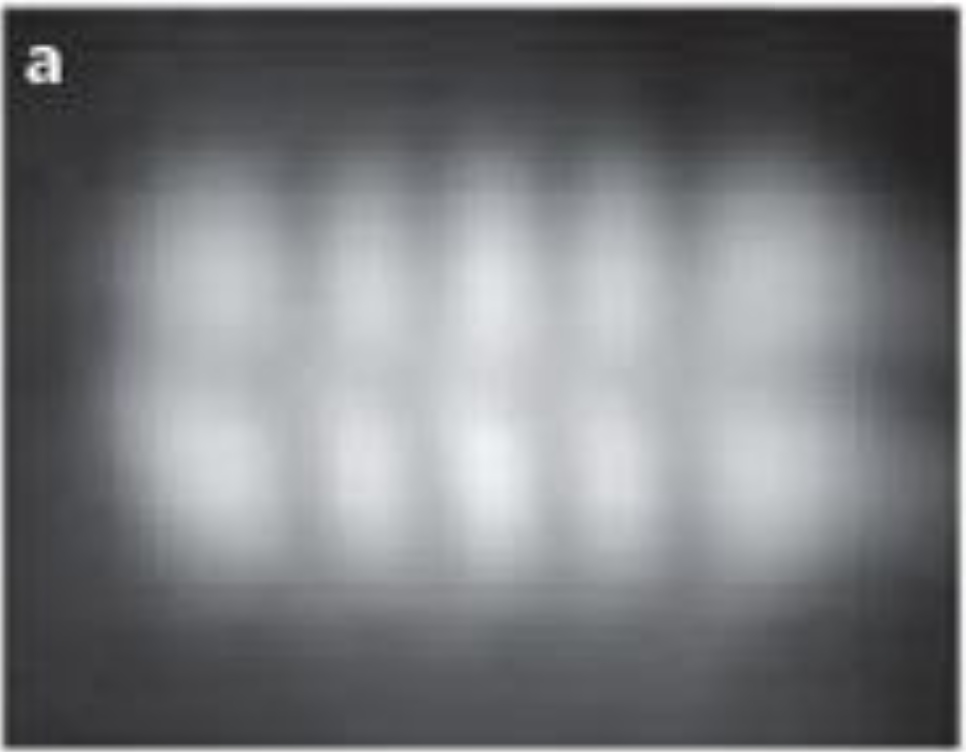
\includegraphics[width=0.8\linewidth]{../ExtFiles/MO-picturea.png}
            \caption{HOMO actual.}
            \label{fig:MO-picturea}
        \end{subfigure}
        \begin{subfigure}[b]{0.3\linewidth}
            \centering
            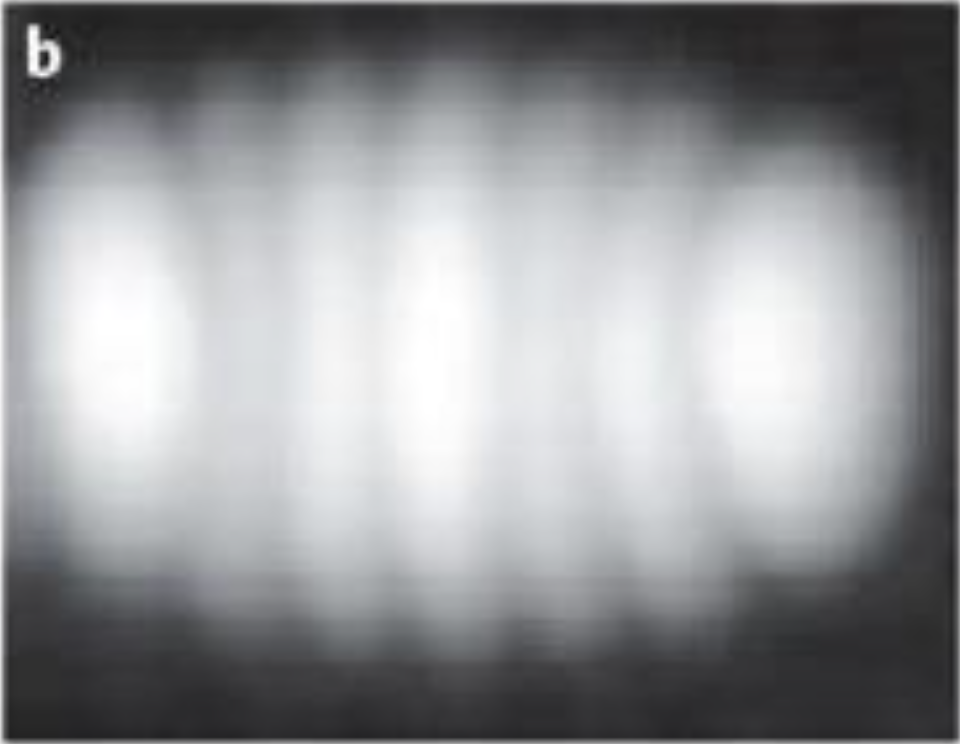
\includegraphics[width=0.8\linewidth]{../ExtFiles/MO-pictureb.png}
            \caption{LUMO actual.}
            \label{fig:MO-pictureb}
        \end{subfigure}
        \begin{subfigure}[b]{0.3\linewidth}
            \centering
            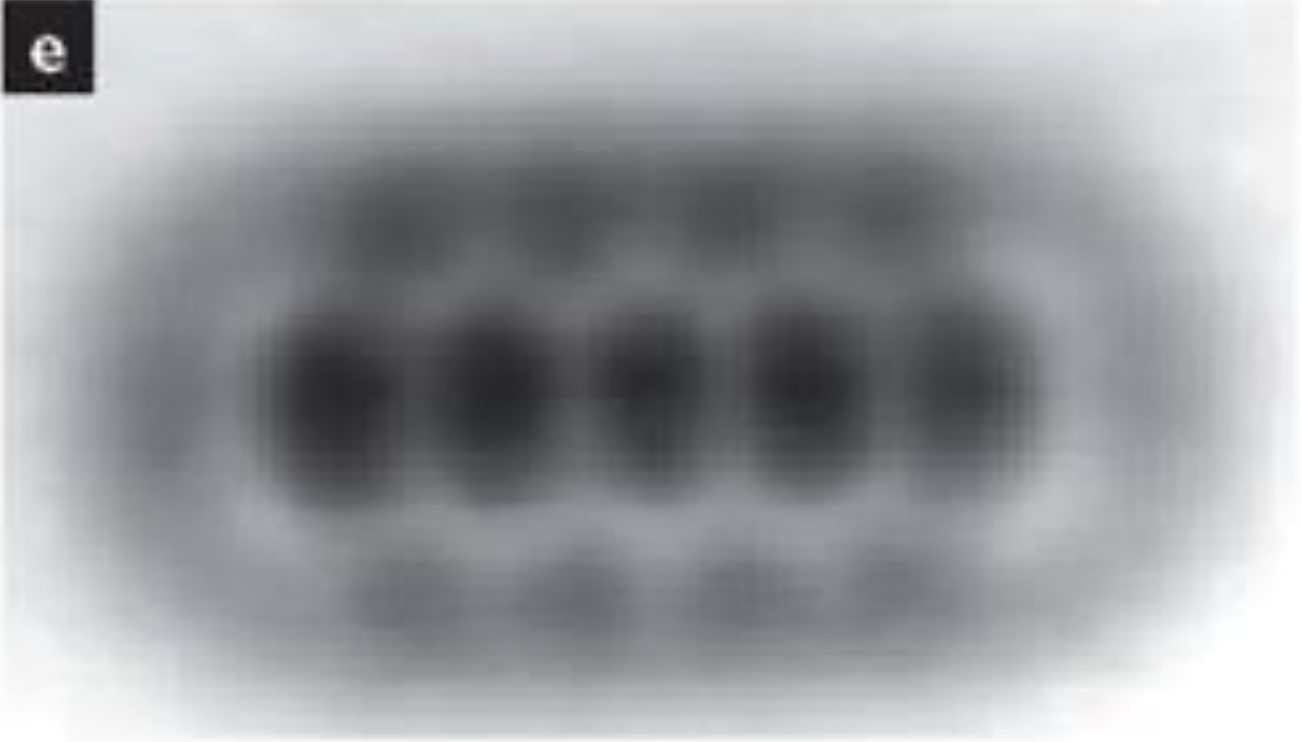
\includegraphics[width=0.8\linewidth]{../ExtFiles/MO-picturec.png}
            \caption{Atomic structure actual.}
            \label{fig:MO-picturec}
        \end{subfigure}\\[1em]
        \begin{subfigure}[b]{0.3\linewidth}
            \centering
            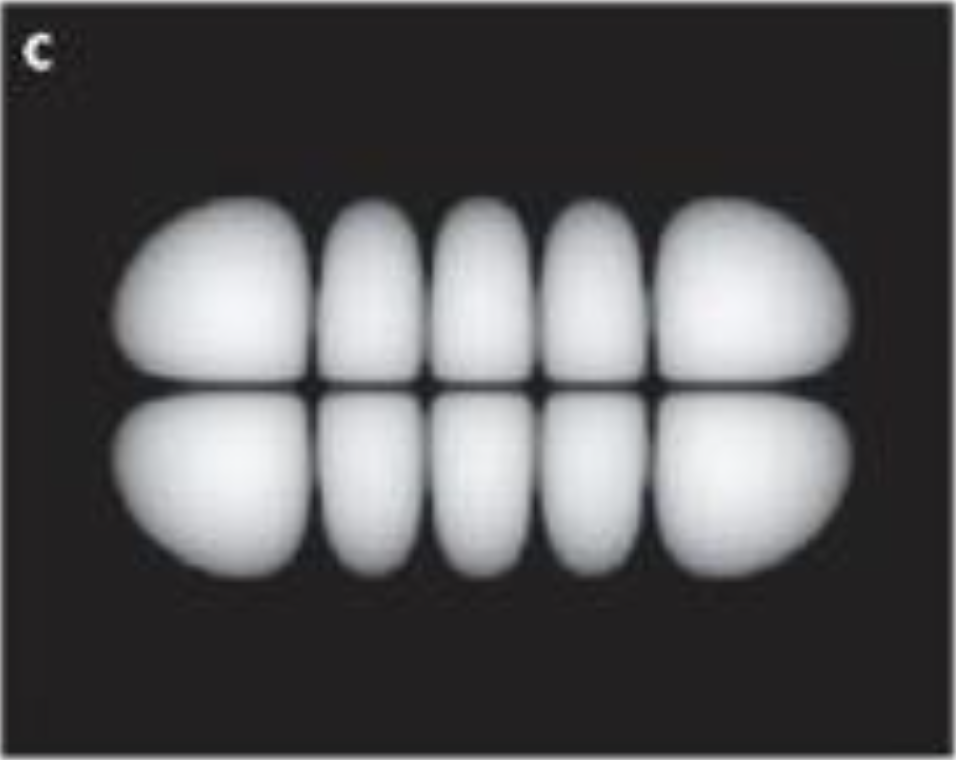
\includegraphics[width=0.8\linewidth]{../ExtFiles/MO-pictured.png}
            \caption{HOMO prediction.}
            \label{fig:MO-pictured}
        \end{subfigure}
        \begin{subfigure}[b]{0.3\linewidth}
            \centering
            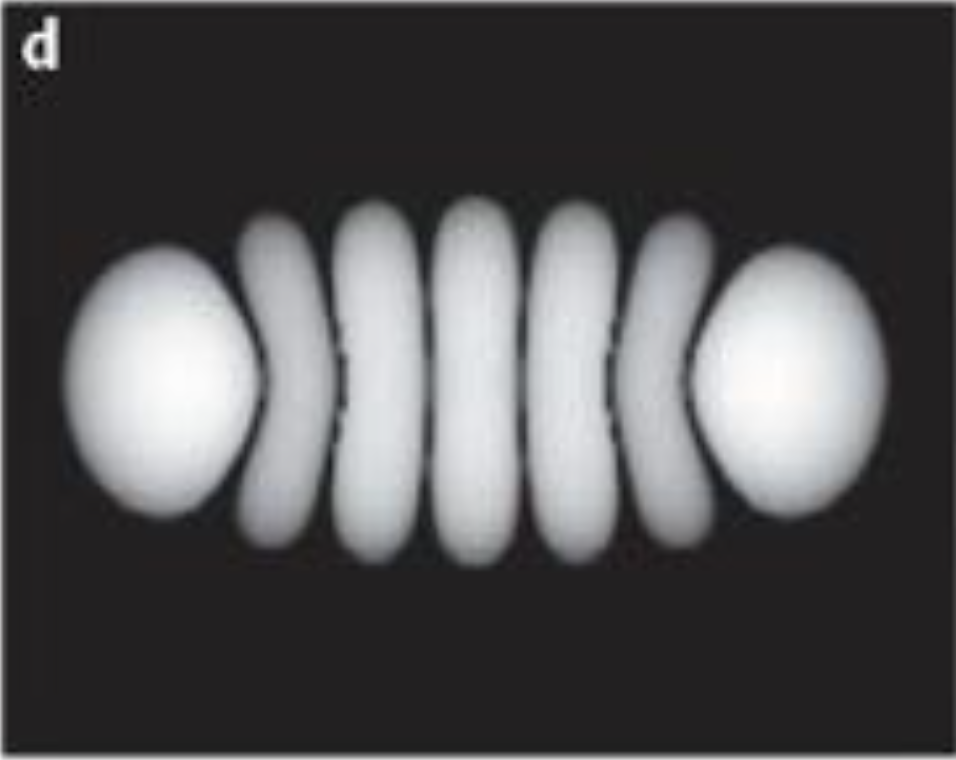
\includegraphics[width=0.8\linewidth]{../ExtFiles/MO-picturee.png}
            \caption{LUMO prediction.}
            \label{fig:MO-picturee}
        \end{subfigure}
        \begin{subfigure}[b]{0.3\linewidth}
            \centering
            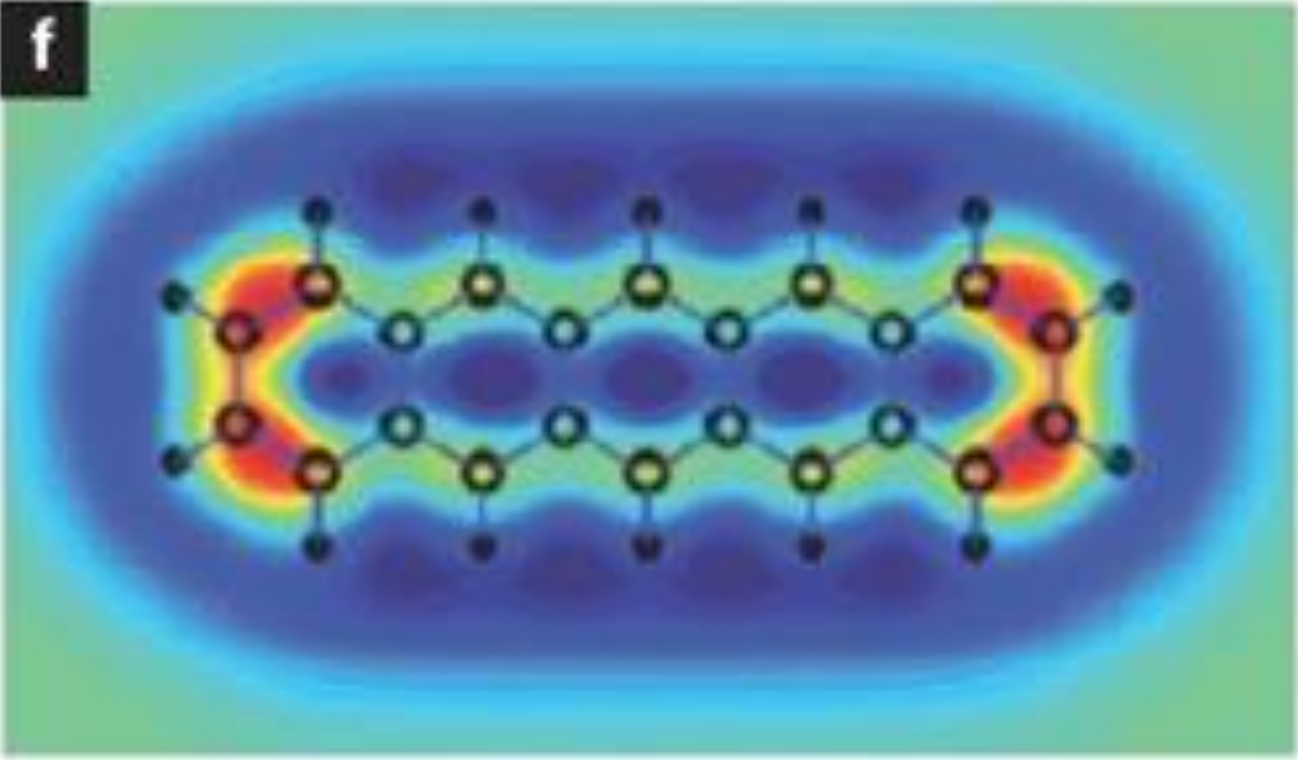
\includegraphics[width=0.8\linewidth]{../ExtFiles/MO-picturef.png}
            \caption{Atomic structure prediction.}
            \label{fig:MO-picturef}
        \end{subfigure}
        \caption{Correspondence between MO predictions and scanning tunnelling microscopy.}
        \label{fig:MO-picture}
    \end{figure}
    \item Can one "see" molecular orbitals? With a scanning tunneling microscope, we can "see" pentatene (5 linearly fused benzene rings). The correspondence between the pictures and MO theory's predictions is impressive (see Figure \ref{fig:MO-picture}).
\end{itemize}



\section{Module 14: Constructing Molecular Orbitals (Part 1)}
\begin{itemize}
    \item Bonding: $\Psi_\sigma=\Psi_+=\frac{1}{\sqrt{2}}(\psi_{1s_a}+\psi_{1s_b})$.
    \item Anti-bonding: $\Psi_{\sigma^*}=\Psi_-=\frac{1}{\sqrt{2}}(\psi_{1s_a}-\psi_{1s_b})$.
    \begin{itemize}
        \item Addition doesn't necessarily correlate to bonding and subtraction to anti-bonding.
    \end{itemize}
    \item With simple orbitals, we can combine orbitals by inspection.
    \begin{itemize}
        \item However, we will learn to build molecular orbitals for much more complicated molecular orbitals, such as those of ferrocene (\ce{Fe(C5H5)2}).
    \end{itemize}
    \item Degree of orbital overlap/mixing depends on:
    \begin{enumerate}
        \item Energy of the orbitals (the closer the energy, the more mixing; when the energies differ greatly, the reduction energy due to bonding is insignificant).
        \item Spatial proximity (the atoms must be close enough that there is \emph{reasonable} orbital overlap, but not so close that repulsive forces interfere).
        \item Symmetry (atomic orbitals mix if they have similar symmetries; regions with the same sign of $\Psi$ overlap).
    \end{enumerate}
    \item The strength of the bond depends upon the degree of orbital overlap.
    \item For heteronuclear molecules:
    \begin{figure}[h!]
        \centering
        \begin{subfigure}[b]{0.33\linewidth}
            \centering
            \begin{tikzpicture}[scale=0.8]
                \footnotesize
                \draw [ultra thick]
                    (-2.3,0) -- node[below=1.62cm]{\ce{A}} (-1.5,0)
                    (1.5,0) -- node[below=1.62cm]{\ce{A}} (2.3,0)
                    (-0.4,-2) -- node[below]{\ce{A-A}} (0.4,-2)
                    (-0.4,3) -- (0.4,3)
                ;
    
                \draw [grx,thick,densely dashed]
                    (-1.5,0) -- (-0.4,-2)
                    (-1.5,0) -- (-0.4,3)
                    (1.5,0) -- (0.4,-2)
                    (1.5,0) -- (0.4,3)
                ;
            \end{tikzpicture}
            \caption{Equal energies.}
            \label{fig:orbitalEnergyCombinationsa}
        \end{subfigure}
        \begin{subfigure}[b]{0.32\linewidth}
            \centering
            \begin{tikzpicture}[scale=0.8]
                \footnotesize
                \draw [ultra thick]
                    (-2.3,0.8) -- node[below=2.25cm]{\ce{A}} (-1.5,0.8)
                    (1.5,-0.3) -- node[below=1.37cm]{\ce{B}} (2.3,-0.3)
                    (-0.4,-2) -- node[below]{\ce{A-B}} (0.4,-2)
                    (-0.4,3) -- (0.4,3)
                ;
    
                \draw [grx,thick,densely dashed]
                    (-1.5,0.8) -- (-0.4,-2)
                    (-1.5,0.8) -- (-0.4,3)
                    (1.5,-0.3) -- (0.4,-2)
                    (1.5,-0.3) -- (0.4,3)
                ;
            \end{tikzpicture}
            \caption{Unequal energies.}
            \label{fig:orbitalEnergyCombinationsb}
        \end{subfigure}
        \begin{subfigure}[b]{0.33\linewidth}
            \centering
            \begin{tikzpicture}[scale=0.8]
                \footnotesize
                \draw [ultra thick]
                    (-2.3,2) -- node[below=3.2cm]{\ce{A}} (-1.5,2)
                    (1.5,-1) -- node[below=0.8cm]{\ce{B}} (2.3,-1)
                    (-0.4,-2) -- node[below]{\ce{A-B}} (0.4,-2)
                    (-0.4,3) -- (0.4,3)
                ;
    
                \draw [grx,thick,densely dashed]
                    (-1.5,2) -- (-0.4,-2)
                    (-1.5,2) -- (-0.4,3)
                    (1.5,-1) -- (0.4,-2)
                    (1.5,-1) -- (0.4,3)
                ;
            \end{tikzpicture}
            \caption{Very unequal energies.}
            \label{fig:orbitalEnergyCombinationsc}
        \end{subfigure}
        \caption{Combining orbitals of varying energies.}
        \label{fig:orbitalEnergyCombinations}
    \end{figure}
    \begin{itemize}
        \item The bonding orbital(s) will reside predominantly on the atom of lower orbital energy (the more electronegative atom).
        \item The anti-bonding orbital(s) will reside predominantly on the atom with greater orbital energy (the less electronegative atom).
    \end{itemize}
    \begin{figure}[h!]
        \centering
        \begin{tikzpicture}[
            xscale=0.52,yscale=0.15,
            pointr/.style={circle,draw,fill=white,thin,inner sep=2pt,label={[xshift=-2pt,yshift=-2pt]85:\ce{#1}}},
            pointa/.style={circle,draw,fill=white,thin,inner sep=2pt,label={[xshift=4pt,yshift=-2pt]90:\ce{#1}}}
        ]
            \small
            \draw (0,0) -- (20,0) -- (20,-50) -- node[below=7mm]{Atomic number} (0,-50) -- node[rotate=90,left=1.3cm,anchor=center]{Potential energy (eV)} cycle;
            \footnotesize
            \foreach \x in {0,5,...,20} {
                \draw (\x,-50) -- ++(0,-1.3) node[below]{$\x$};
            }
            \foreach \y in {0,-10,...,-50} {
                \draw (0,\y) -- ++(-0.4,0) node[left]{$\y$};
            }
    
            \foreach \val/\atom [count=\x from 2,remember=\x as \lastx (initially 1),remember=\val as \lastval (initially -13.61),remember=\atom as \lastatom (initially H)] in {-24.59/He} {
                \draw [thick] (\lastx,\lastval) node[pointr=\lastatom]{} -- (\x,\val);
            }
            \node [pointr=He] at (2,-24.59) {};
            \foreach \val/\atom [count=\x from 4,remember=\x as \lastx (initially 3),remember=\val as \lastval (initially -5.39),remember=\atom as \lastatom (initially Li)] in {-9.32/Be,-14.05/B,-19.43/C,-25.56/N,-32.38/O,-40.17/F,-48.47/Ne} {
                \draw [thick] (\lastx,\lastval) node[pointr=\lastatom]{} -- (\x,\val);
            }
            \node [pointr=Ne] at (10,-48.47) {};
            \foreach \val/\atom [count=\x from 6,remember=\x as \lastx (initially 5),remember=\val as \lastval (initially -8.30),remember=\atom as \lastatom (initially B)] in {-10.66/C,-13.18/N,-15.85/O,-18.65/F,-21.59/Ne} {
                \draw [thick] (\lastx,\lastval) node[pointr=\lastatom]{} -- (\x,\val);
            }
            \node [pointr=Ne] at (10,-21.59) {};
            \foreach \val/\atom [count=\x from 12,remember=\x as \lastx (initially 11),remember=\val as \lastval (initially -5.14),remember=\atom as \lastatom (initially Na)] in {-7.65/Mg,-11.32/Al,-15.89/Si,-18.84/P,-22.71/S,-25.23/Cl,-29.24/Ar} {
                \draw [thick] (\lastx,\lastval) node[pointa=\lastatom]{} -- (\x,\val);
            }
            \node [pointa=Ar] at (18,-29.24) {};
            \foreach \val/\atom [count=\x from 14,remember=\x as \lastx (initially 13),remember=\val as \lastval (initially -5.98),remember=\atom as \lastatom (initially Al)] in {-7.78/Si,-9.65/P,-11.62/S,-13.67/Cl,-15.82/Ar} {
                \draw [thick] (\lastx,\lastval) node[pointa=\lastatom]{} -- (\x,\val);
            }
            \node [pointa=Ar] at (18,-15.82) {};

            \draw [semithick,grx,-stealth] (3,-17) node[right,black]{$1s$} -- (1.7,-19);
            \draw [semithick,grx,-stealth] (5,-26) node[left,black]{$2s$} -- (6.3,-22);
            \draw [semithick,grx,-stealth] (10,-11) node[right,black]{$2p$} -- (8.6,-17);
            \draw [semithick,grx,-stealth] (13,-22) node[left,black]{$3s$} -- (14.3,-17.5);
            \draw [semithick,grx,-stealth] (18.5,-9) node[right,black]{$3p$} -- (17.6,-14.3);
        \end{tikzpicture}
        \caption{Orbital potential energies.}
        \label{fig:orbitalPotentialEnergies}
    \end{figure}
    \item The energies of atomic orbitals (measured by PES) have been tabulated (see Figure \ref{fig:orbitalPotentialEnergies}).
    \item If you want to measure orbital energies in the range of -10 eV (i.e., upper valence orbitals; see Table 5.2 in \textcite{bib:MiesslerFischerTarr}), use UPS. If you want to look at energy states that are very deep, very core (i.e., $1s$ in \ce{Fe}), use XPS.
    \item \textbf{State conservation principle}: The number of molecular orbitals is equal to the number of incipient (atomic) orbitals.
    \item Symmetry and orbital diagrams (suggested reading \textcite{bib:reinforceMOTheory}):
    \begin{itemize}
        \item Orbitals of the same symmetry mix.
        \item Orbital interactions can be bonding, nonbonding, or antibonding.
        \item There are three basic types of orbital overlap: $\sigma$ (end-on interaction), $\pi$ (side-by-side approach) and $\delta$ (off-axis approach).
        \begin{itemize}
            \item $\sigma$ orbitals are symmetric to rotation about the line connecting nuclei.
            \item $\pi$ orbitals change sign of the wave function with $C_2$ rotation about the bond axis.
            \item Orbitals also denoted $g$ are symmetric to inversion.
            \item Orbitals also denoted $u$ are antisymmetric to inversion.
        \end{itemize}
        \item Orbitals with the correct symmetry and most similar energy mix to the greatest extent.
    \end{itemize}
    \begin{figure}[h!]
        \centering
        \begin{subfigure}[b]{0.63\linewidth}
            \centering
            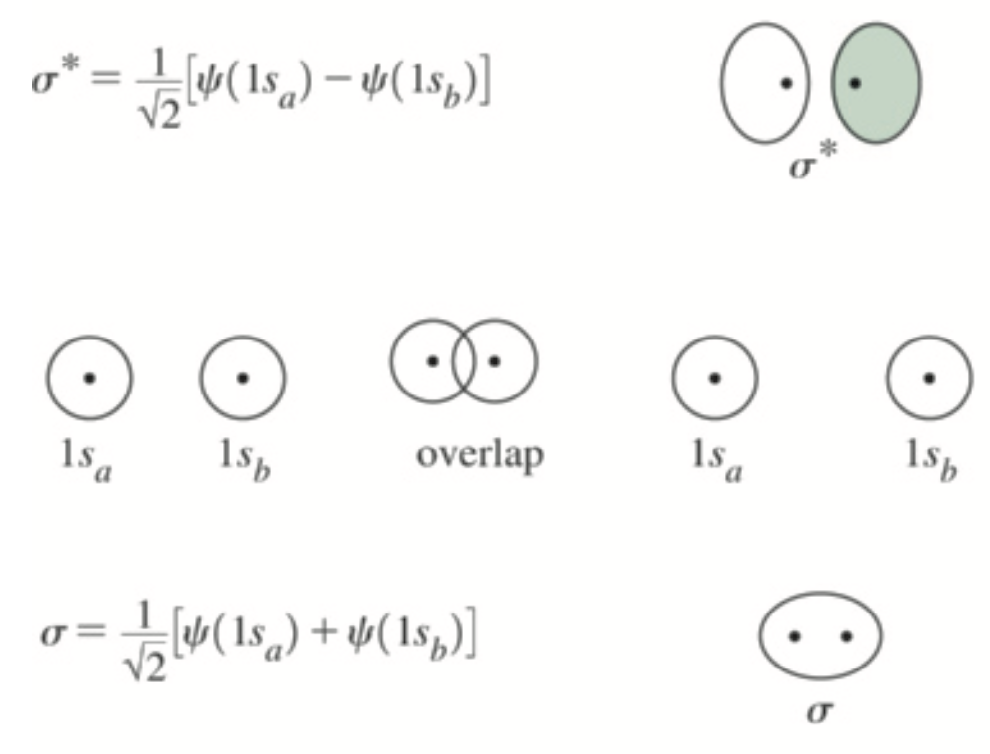
\includegraphics[width=0.8\linewidth]{../ExtFiles/constructingMOsa.png}
            \caption{$\sigma_s$.}
            \label{fig:constructingMOsa}
        \end{subfigure}
    \end{figure}
    \begin{figure}[h!]\ContinuedFloat
        \centering
        \begin{subfigure}[b]{0.49\linewidth}
            \centering
            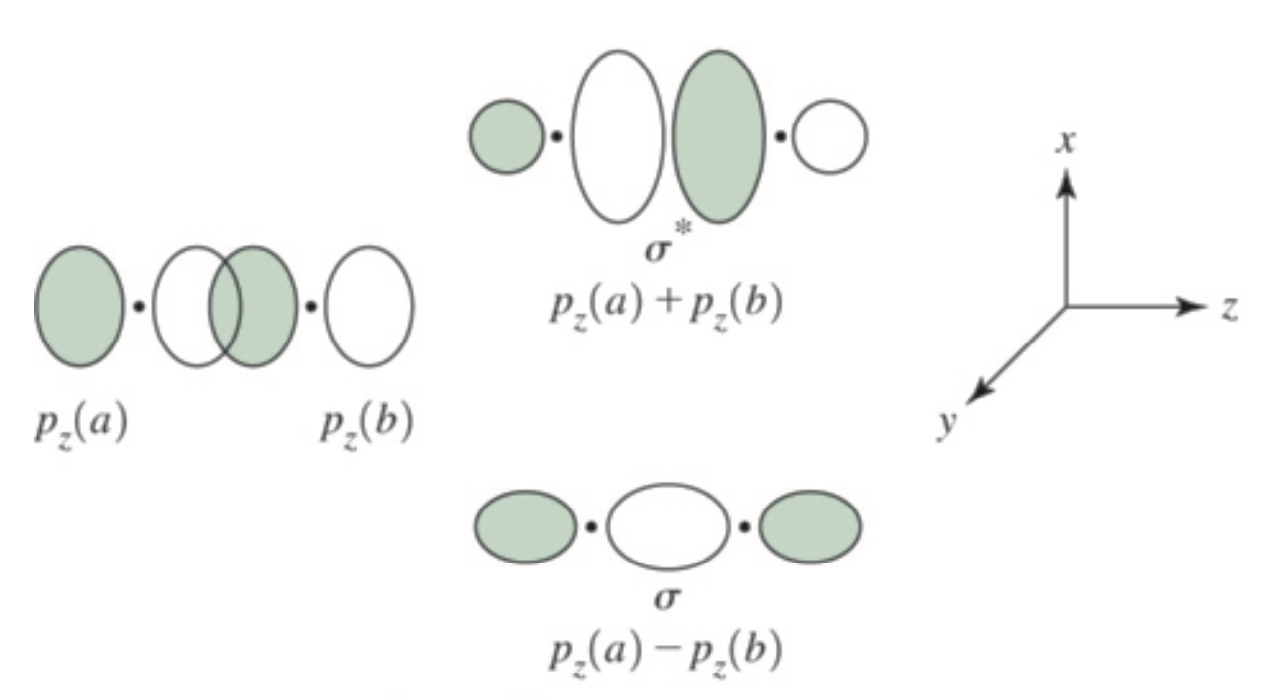
\includegraphics[width=0.9\linewidth]{../ExtFiles/constructingMOsb.png}
            \caption{$\pi_s$.}
            \label{fig:constructingMOsb}
        \end{subfigure}
        \begin{subfigure}[b]{0.49\linewidth}
            \centering
            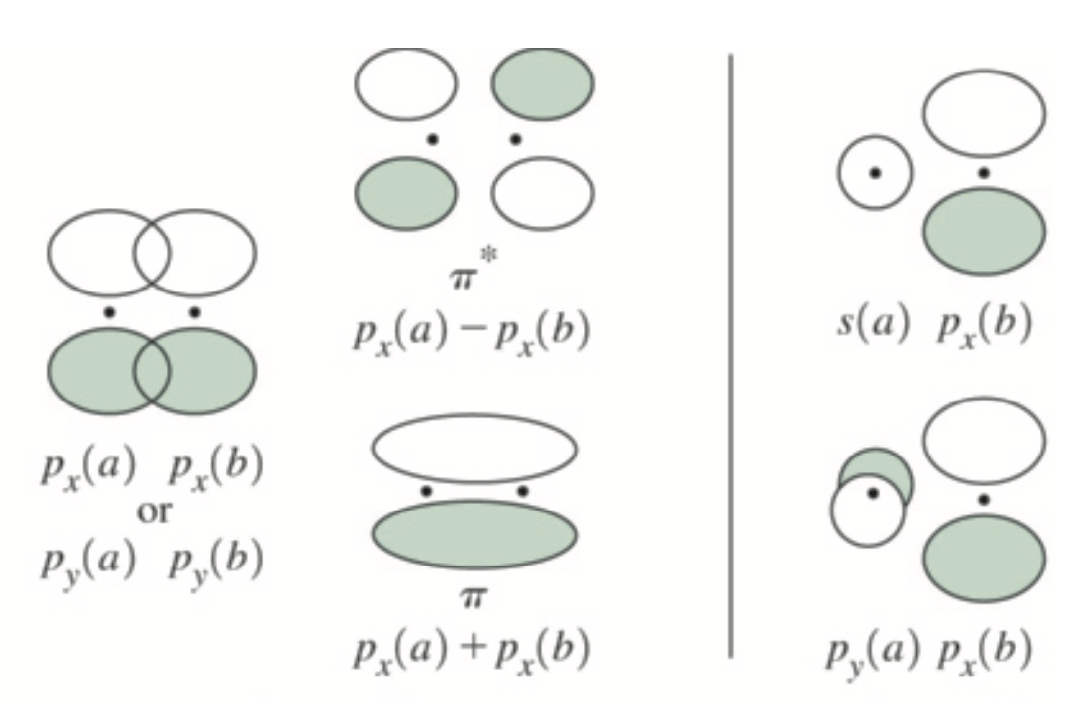
\includegraphics[width=0.9\linewidth]{../ExtFiles/constructingMOsc.png}
            \caption{$\pi_p$.}
            \label{fig:constructingMOsc}
        \end{subfigure}\\[1em]
        \begin{subfigure}[b]{\linewidth}
            \centering
            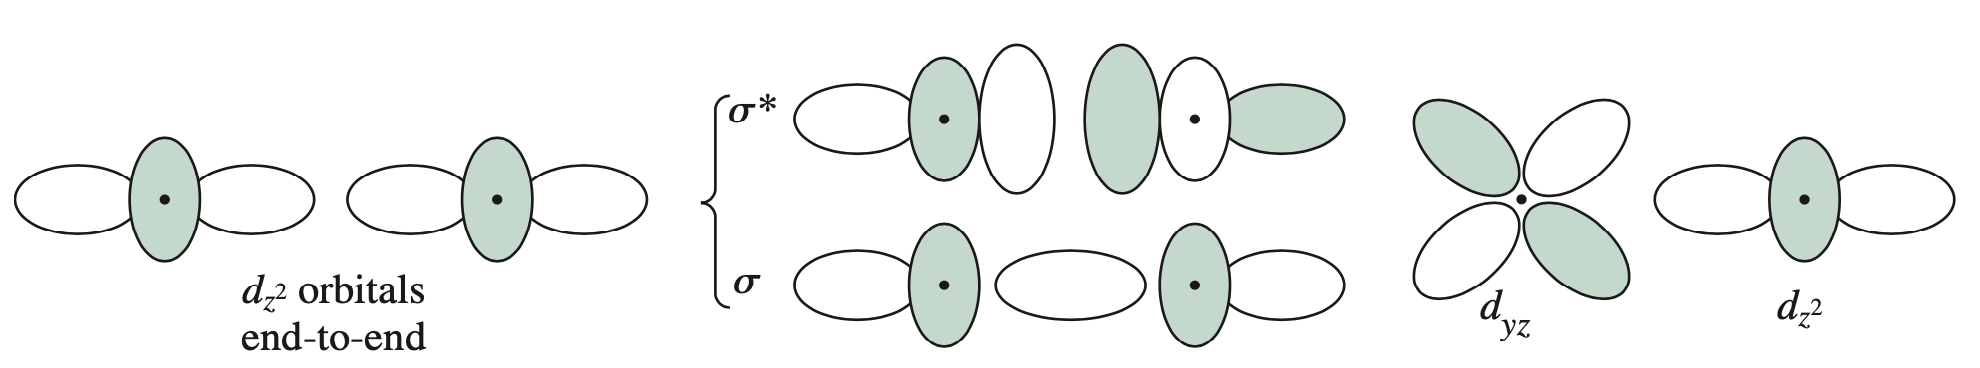
\includegraphics[width=0.8\linewidth]{../ExtFiles/constructingMOsd.png}
            \caption{$\delta_s$.}
            \label{fig:constructingMOsd}
        \end{subfigure}\\[1em]
        \begin{subfigure}[b]{\linewidth}
            \centering
            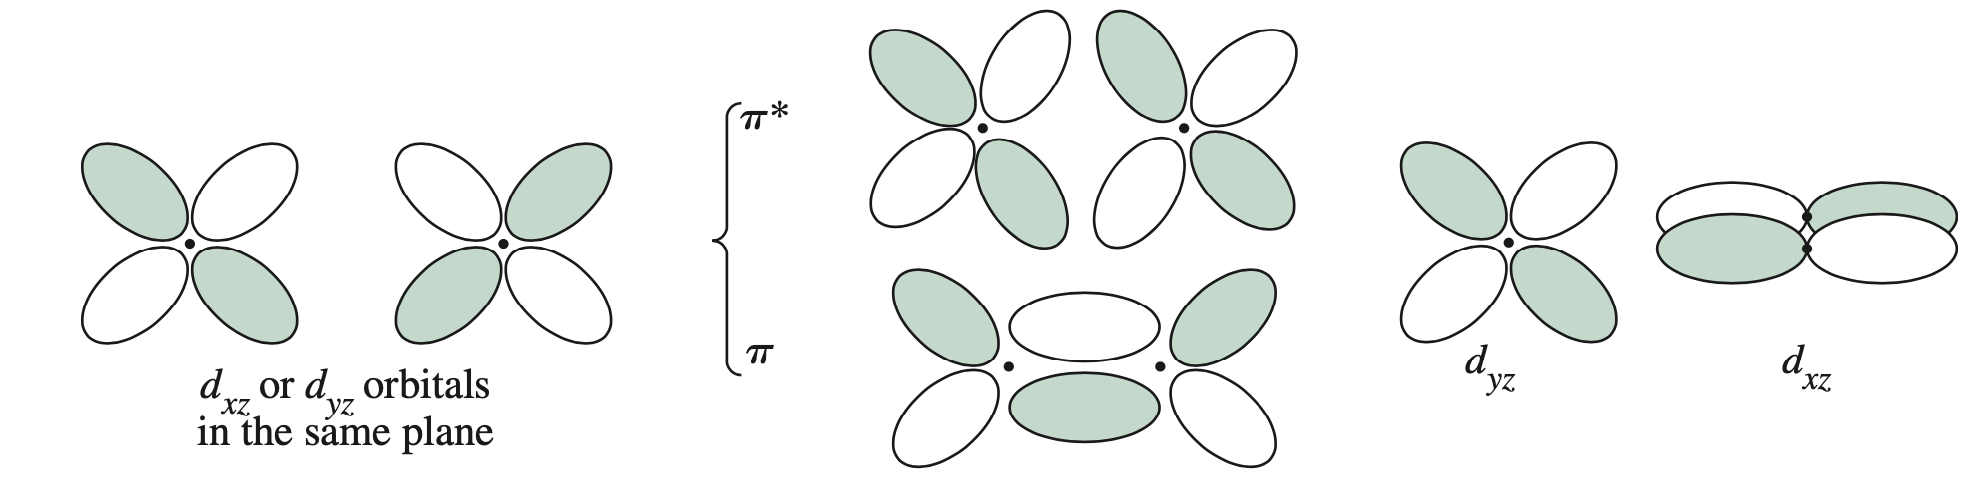
\includegraphics[width=0.8\linewidth]{../ExtFiles/constructingMOse.png}
            \caption{$\delta_p$.}
            \label{fig:constructingMOse}
        \end{subfigure}\\[1em]
        \begin{subfigure}[b]{\linewidth}
            \centering
            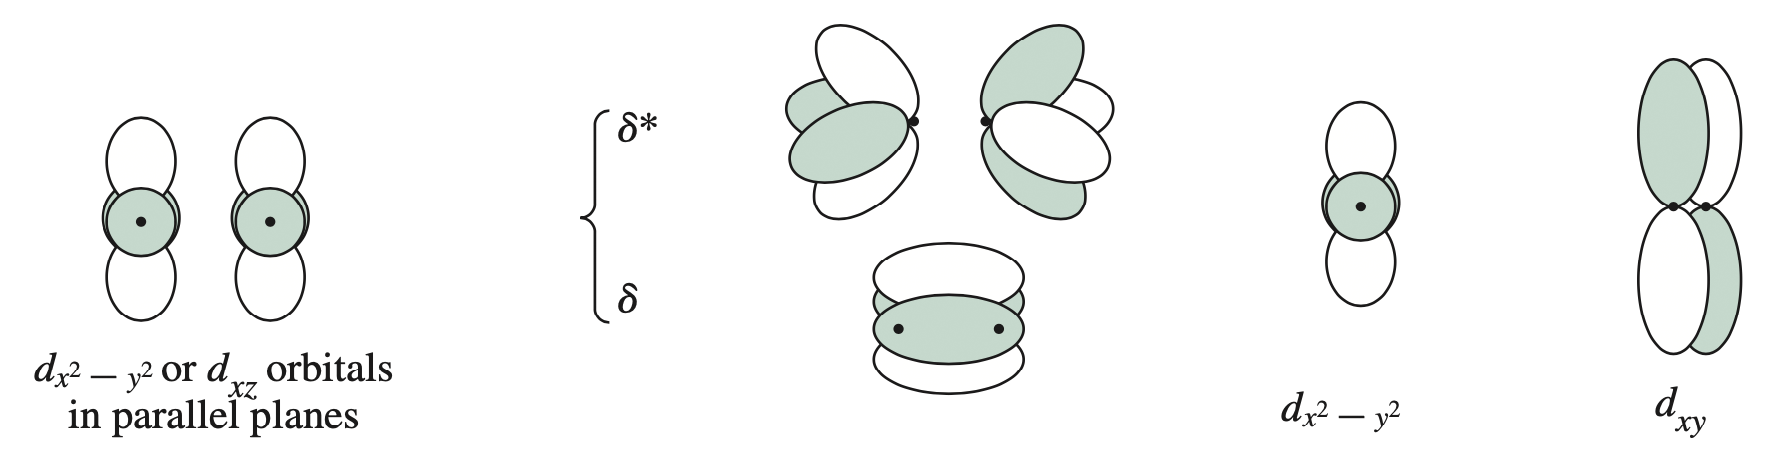
\includegraphics[width=0.8\linewidth]{../ExtFiles/constructingMOsf.png}
            \caption{$\delta_d$.}
            \label{fig:constructingMOsf}
        \end{subfigure}
        \caption{Constructing $s$, $p$, and $d$ molecular orbitals.}
        \label{fig:constructingMOs}
    \end{figure}
    \item There are six MO constructions to be aware of: $s$-$s$, $p$-$p$ ($\sigma$ and $\pi$), and $d$-$d$ ($\sigma$, $\pi$, and $\delta$). See Figure \ref{fig:constructingMOs}.
    \begin{itemize}
        \item There are similar orbitals in simple diatomic molecules.
    \end{itemize}
    \item As the mixing of $\sigma_g$ orbitals gets stronger, the $2p$ state drops in energy faster than the $2s$ state, causing the $2p$ state to have lower energy than the $2s$ state after a while.
\end{itemize}



\section{Office Hours (Wang)}
\begin{itemize}
    \item Quantum mechanics will not be included on tomorrow's exam.
    \item Hybridization was developed (1931 by Pauling) earlier than VSEPR theory (1940 by Sidgwick and Powell).
    \item What \emph{is} a direct product of representations?
    \begin{itemize}
        \item The direct product generates an $n\times m$ matrix?
        \item Di doesn't have a great explanation, but he's gonna give me a link to his Advanced Inorganic Chemistry textbook.
    \end{itemize}
    \item Can you go over how to do problems IV and VI with direct product analysis?
    \begin{itemize}
        \item The IR absorption way from Module 12?
        \item $\Gamma_\text{g.s.}=A_1$ always.
        \item $\Gamma_\mu$ is the sum of the $x,y,z$ linear irreducible representations.
        \item $\Gamma_\text{e.s.}=\Gamma_\text{vibs}$.
        \item We need to calculate the direct product of every representation in $\Gamma_\text{vibs}$ with every term in $\Gamma_\mu$. Products that contain $A_1$ are IR active?
        \item Example:
        \begin{equation*}
            A_1\times(A_1+B_1+B_1) = A_1\times A_1+A_1\times B_1+A_1\times B_2
        \end{equation*}
        \begin{itemize}
            \item Since $A_1\times A_1=A_1$, we already know after taking only this product that $A_1$ is IR active.
        \end{itemize}
        \item Things aren't IR active because they're linear. Things are IR active because their direct product with the sum of the linear groups contains the totally symmetric representation.
    \end{itemize}
    \item You can only take the direct product of irreducible representations?
\end{itemize}



\section{Office Hours (Talapin)}
\begin{itemize}
    \item To what extent do we need to know term symbols (they appeared briefly in Module 1)?
    \item How do we identify the $T_h$ point group?
    \begin{figure}[h!]
        \centering
        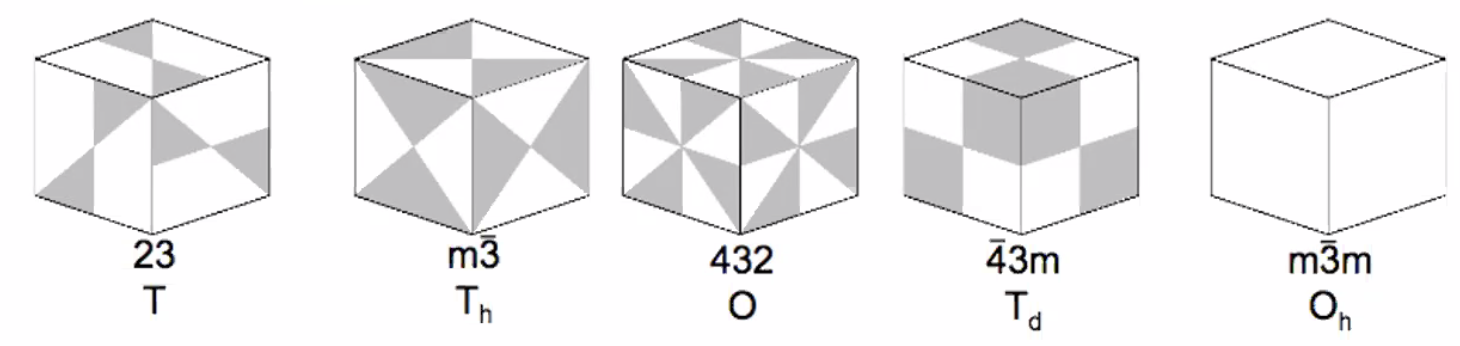
\includegraphics[width=0.7\linewidth]{../ExtFiles/tetrahedralPGs.png}
        \caption{Tetrahedral point groups.}
        \label{fig:tetrahedralPGs}
    \end{figure}
    \begin{itemize}
        \item It's a very rare point group. It has no dihedral planes.
    \end{itemize}
    \item What is the point of conjugate elements?
    \begin{itemize}
        \item Conjugate elements allow us to group symmetry elements into classes --- conjugate elements are in the same class!
    \end{itemize}
    \item Will we need to be able to work with infinite character tables?
    \item What was that whole thing you did with a symmetry operation $R$ and the Schr\"{o}dinger equation?
    \item What level of familiarity do we need with Dirac's bra-ket notation?
    \begin{itemize}
        \item Just know that it represents an integral.
    \end{itemize}
    \item Do we need to evaluate/what do we need to know about those integrals from Wednesday's class?
    \begin{itemize}
        \item It will be sufficient to write down representations.
    \end{itemize}
    \item Why does $\Gamma_\mu$, the representation of the dipole moment, transform with $x,y,z$?
    \begin{itemize}
        \item $n$-degree perturbation theory.
    \end{itemize}
    \item The problems will be similar to homework problems.
\end{itemize}



\section{Module 15: Constructing Molecular Orbitals (Part 2, \ce{HF} Molecule)}
\begin{itemize}
    \item \marginnote{2/1:}MO Diagrams from Group Theory:
    \begin{enumerate}
        \item Assign a point group.
        \item Choose basis functions (orbitals).
        \item Apply operations.
        \item Generate (a) reducible representation(s) and SALCs (the latter if applicable).
        \item Reduce to irreducible representations.
        \item Combine central and peripheral orbitals by their symmetry.
        \item Fill MOs with $\e[-]$'s. Draw orbitals.
        \item Generate SALCs of peripheral atoms (if applicable).
        \item Draw peripheral atom SALC with central atom orbital to generate bonding/antibonding MOs (if applicable).
    \end{enumerate}
    \item We will not need SALCs here.
    \item \ce{H-F} example:
    \begin{itemize}
        \item Point group: $C_{\infty v}$. However, we will work within the $C_{2v}$ subgroup (knowing why to choose this \emph{specific} subgroup will come later; just accept it for now).
        \item Choose basis functions (\ce{H_{$1s$}}, \ce{F_{$1s$}}, \ce{F_{$2p_x$}}, \ce{F_{$2p_y$}}, and \ce{F_{$2p_z$}}).
        \item Applying operations, we get
        \begin{align*}
            \Gamma_{\ce{H_{1s}}} &= (1,1,1,1) = A_1\\
            \Gamma_{\ce{F_{1s}}} &= (1,1,1,1) = A_1\\
            \Gamma_{\ce{F_{2p_z}}} &= (1,1,1,1) = A_1\\
            \Gamma_{\ce{F_{2p_x}}} &= (1,-1,1,-1) = B_1\\
            \Gamma_{\ce{F_{2p_y}}} &= (1,-1,-1,1) = B_2
        \end{align*}
        \begin{itemize}
            \item Therefore, the \ce{H_{$1s$}}, \ce{F_{$1s$}}, \ce{F_{$2p_x$}}, \ce{F_{$2p_y$}}, and \ce{F_{$2p_z$}} orbitals transform with the $A_1$, $A_1$, $A_1$, $B_1$, and $B_2$ irreducible representations, respectively.
            \item Note that we can also extract $p$-orbital information from the corresponding linear functions in the character table.
            \item Also note that one orbital $\Rightarrow$ one degree of freedom. We do not have $x,y,z$-DOFs as before.
        \end{itemize}
        \item When we bring the atoms together, those orbitals with similar symmetry (in this case, all the $A_1$ orbitals) will start mixing. However, from Figure \ref{fig:orbitalPotentialEnergies}, the \ce{F_{$1s$}} orbital has a very different energy (much lower) than the \ce{H_{$1s$}} orbital, meaning that it has negligible mixing with \ce{H_{$1s$}}. On the other hand, \ce{H_{$1s$}} along with the $2p$-orbitals in fluorine have comparable energies, so they will have significant mixing.
        \item We will get a low energy MO from \ce{F_{$1s$}}, a higher bonding MO from \ce{H_{$1s$}} and \ce{F_{$2p_z$}}, two higher nonbonding MOs from \ce{F_{$2p_x$}} and \ce{F_{$2p_y$}}, and a higher anti-bonding MO from \ce{H_{$1s$}} and \ce{F_{$2p_z$}}.
        \begin{figure}[H]
            \centering
            \begin{subfigure}[b]{0.45\linewidth}
                \centering
                \begin{tikzpicture}[
                    yscale=0.15,
                    every node/.prefix style={black}
                ]
                    \footnotesize
                    \draw [ultra thick,gry] (2,-40.17) -- node{\Large$\upharpoonleft$\hspace{-1mm}$\downharpoonright$} node[below=2mm]{$2s(A_1)$} ++(0.5,0);
                    \draw [ultra thick,gry] (2,-18.65) -- node{\Large$\upharpoonleft$\hspace{-1mm}$\downharpoonright$} node[below=2mm]{$p_z(A_1)$} ++(0.5,0) ++(0.1,0) -- node{\Large$\upharpoonleft$\hspace{-1mm}$\downharpoonright$} node[below=7mm]{$p_y(B_2)$} ++(0.5,0) ++(0.1,0) -- node{\Large$\upharpoonleft$} node[below=2mm]{$p_x(B_1)$} ++(0.5,0);
                    \draw [ultra thick,gry] (-2.5,-13.61) -- node{\Large$\upharpoonleft$} node[below=2mm]{$1s(A_1)$} ++(0.5,0);
            
                    \draw [ultra thick] (-0.55,-40.17) -- node{\Large$\upharpoonleft$\hspace{-1mm}$\downharpoonright$} node[below=2mm]{$a_1$} ++(1.1,0);
                    \draw [ultra thick] (-0.55,-28) -- node{\Large$\upharpoonleft$\hspace{-1mm}$\downharpoonright$} node[below=2mm]{$a_1$} ++(1.1,0);
                    \draw [ultra thick] (-0.55,-18.65) -- node{\Large$\upharpoonleft$\hspace{-1mm}$\downharpoonright$} node[below=2mm,xshift=-2mm]{$p_y(b_2)$} ++(0.5,0) (0.05,-18.65) -- node{\Large$\upharpoonleft$\hspace{-1mm}$\downharpoonright$} node[below=2mm,xshift=2mm]{$p_x(b_1)$} ++(0.5,0);
                    \draw [ultra thick] (-0.55,-7) -- node[below]{$A_1$} ++(1.1,0);
            
                    \draw [grx,densely dashed]
                        (-2,-13.61) -- (-0.55,-7)
                        (-2,-13.61) -- (-0.55,-28)
                        (2,-18.65) -- (0.55,-7)
                        (2,-18.65) -- (0.55,-28)
                        (2,-40.17) -- (0.55,-40.17)
                        (2,-18.65) -- (0.55,-18.65)
                    ;
                \end{tikzpicture}
                \caption{Energy level diagram.}
                \label{fig:orbitalDiagram-HFa}
            \end{subfigure}
            \begin{subfigure}[b]{0.45\linewidth}
                \centering
                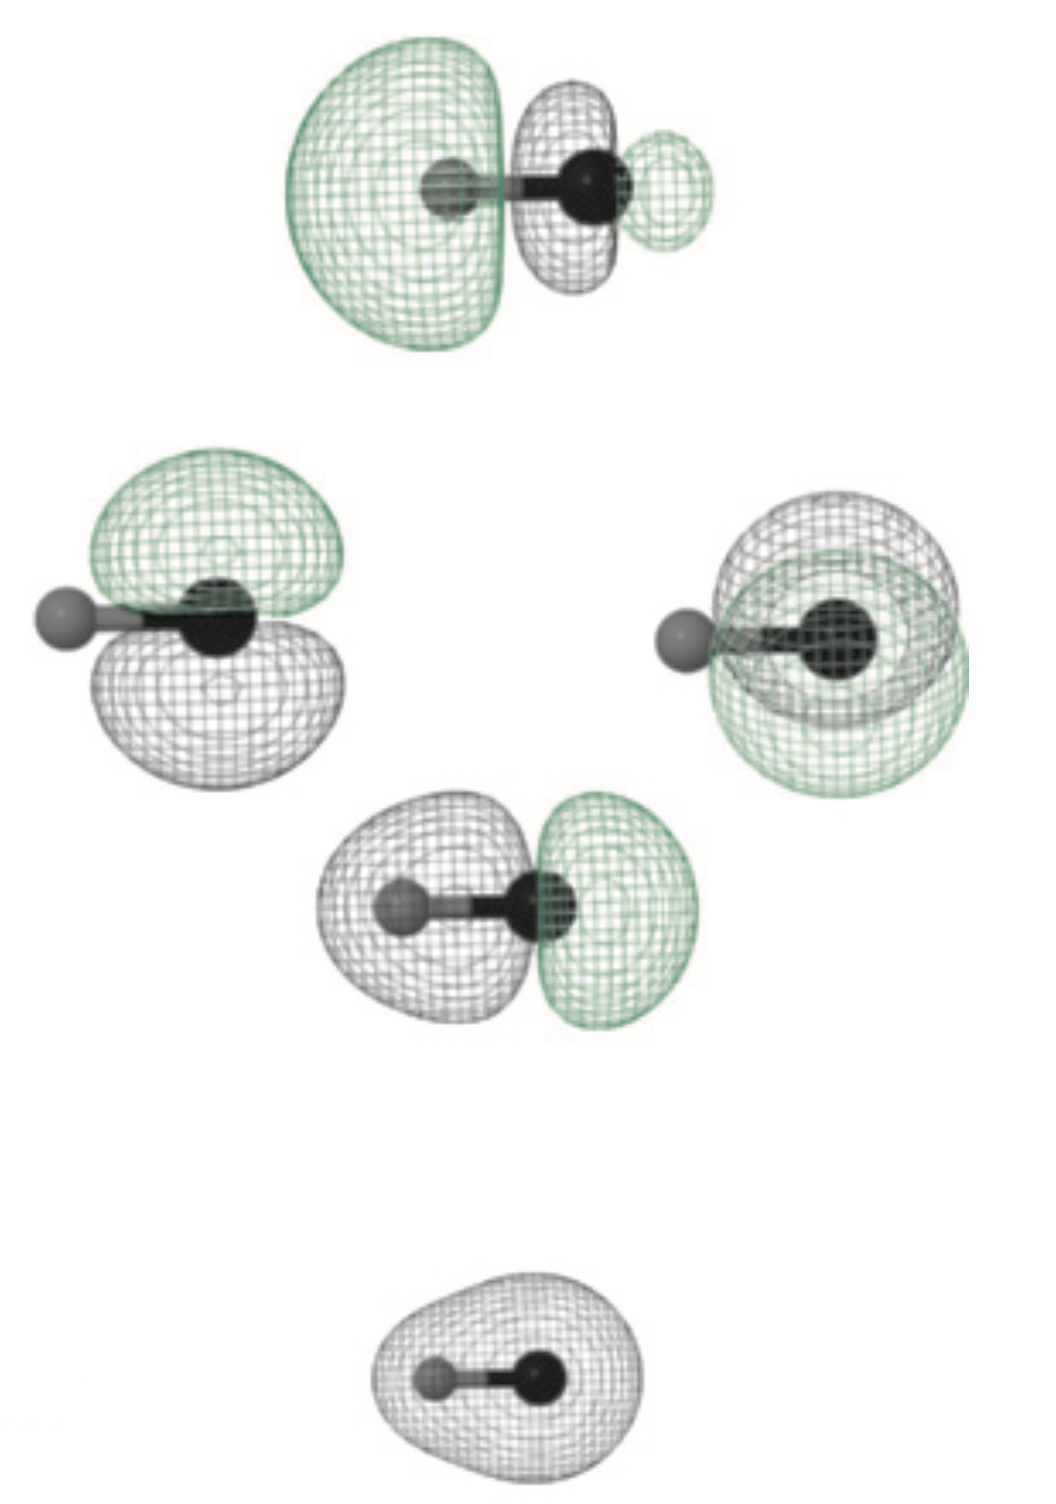
\includegraphics[width=0.6\linewidth]{../ExtFiles/orbitalDiagram-HFb.png}
                \caption{Orbital drawings.}
                \label{fig:orbitalDiagram-HFb}
            \end{subfigure}
            \caption{\ce{HF} orbital diagram.}
            \label{fig:orbitalDiagram-HF}
        \end{figure}
        \item We can now fill the MOs with the atomic electrons using the Aufbau principle, the Pauli exclusion principle, and Hund's rule. We can also draw these orbitals.
    \end{itemize}
    \item Orbital energies can be found in Table 5.2 of \textcite{bib:MiesslerFischerTarr}.
    \item If the energy difference between orbitals is more than $\SI{10}{eV}$, then we can \emph{probably} (not always) ignore mixing.
    \begin{itemize}
        \item The approximate scaling is that the stabilization energy (or energy gain) is inversely proportional to the energy gap.
        \item The magnitude of the interaction integral will be approximately inversely proportional to the energy gap between the atomic orbitals participating.
    \end{itemize}
    \item Organic chemists can go a long way with a hybridization approach even though it is not reflected in inorganic chemistry.
\end{itemize}



\section{Module 16: Constructing Molecular Orbitals (Part 3, \ce{H2O} Molecule)}
\begin{itemize}
    \item Beware: Orientation of the point groups $C_{2v}$ and $D_{2h}$.
    \begin{itemize}
        \item Unlike all other groups, $C_{2v}$ and $D_{2h}$ present problems in assigning the irreducible representations. For most groups, the symmetry axis is obvious, or if their are several axes, the principal axis is obvious. For $C_{2v}$ and $D_{2h}$, an ambiguity exists. The commonly (but not unanimously) used convention is the following:
        \item If there are three $C_2$ axes, the one with the largest number of atoms unmoved by a $C_2$ operation is $z$. If there is only one $C_2$ axis, that is $z$.
        \item Once $z$ is defined, the $y$-axis is defined as the axis of the remaining two axes which has the largest number of atoms unmoved by the $\sigma$ symmetry operation.
        \item The $x$-axis is the remaining axis.
        \item The overall result is that the symmetry axes in ethylene are defined as: $z$ - along the \ce{C=C} bond; $y$ - in the molecular plane, perpendicular to the \ce{C=C} bond; and $x$ - out of the plane.
        \item Similar approaches apply to the $C_{2v}$ point group.
    \end{itemize}
    \item We will need SALCs here.
    \begin{itemize}
        \item Since the hydrogen atoms do not lie on the principal rotation axis, they will not individually obey the symmetry operations.
        \item Thus, we need \textbf{Symmetry Adapted Linear Combinations}.
    \end{itemize}
    \item \textbf{Symmetry Adapted Linear Combination} (of atomic orbitals): The linear combination of multiple atomic orbitals corresponding to peripheral atoms (atoms that do not lie on the principal axis). This linear combination will obey the symmetry modes. \emph{Also known as} \textbf{SALC}.
    \item To generate SALCs, the steps are:
    \begin{itemize}
        \item Group the atomic orbitals in the molecule into sets which are equivalent by symmetry.
        \item Generate and reduce the reducible representation for each set.
        \item Use the projection operator for one basis.
    \end{itemize}
    \item \ce{H2O} example:
    \begin{itemize}
        \item Point group: $C_{2v}$.
        \item Choose basis functions (both \ce{H_{$1s$}} orbitals, \ce{O} the same as \ce{F} in the last example).
        \item Applying operations, we get
        \begin{equation*}
            \Gamma_{\ce{H}} = (2,0,2,0) = A_1+B_1
        \end{equation*}
        \begin{itemize}
            \item For the hydrogens, it makes sense that we need two irreducible representations to describe two atoms. More formally, the number of basis functions should match the number of irreducible representations to account for possible degeneracy of irreducible representations.
            \item The \ce{O} orbitals are the same as the \ce{F} orbitals in the last example.
        \end{itemize}
        \item Combining orbitals by their symmetry and energy again, we get the following MOs.
        \begin{figure}[H]
            \centering
            \begin{tikzpicture}[
                yscale=0.15,
                every node/.prefix style={black}
            ]
                \footnotesize
                \draw [ultra thick,gry] (2,-40.17) -- node{\Large$\upharpoonleft$\hspace{-1mm}$\downharpoonright$} node[below=2mm]{$2s(A_1)$} ++(0.5,0);
                \draw [ultra thick,gry]
                    (2,-15.85) -- node{\Large$\upharpoonleft$\hspace{-1mm}$\downharpoonright$} node[below=2mm]{$p_z(A_1)$} ++(0.5,0)
                    ++(0.1,0) -- node{\Large$\upharpoonleft$} node[below=7mm]{$p_x(B_1)$} ++(0.5,0)
                    ++(0.1,0) -- node{\Large$\upharpoonleft$} node[below=2mm]{$p_y(B_2)$} ++(0.5,0)
                ;
                \draw [ultra thick,gry]
                    (-3.1,-13.61) -- node{\Large$\upharpoonleft$} node[below=2mm]{$A_1$} ++(0.5,0)
                    (-2.5,-13.61) -- node{\Large$\upharpoonleft$} node[below=2mm]{$B_1$} ++(0.5,0)
                ;
        
                \draw [ultra thick] (-0.55,-44) -- node{\Large$\upharpoonleft$\hspace{-1mm}$\downharpoonright$} node[below=2mm]{$a_1$} ++(1.1,0);
                \draw [ultra thick] (-0.55,-34) -- node{\Large$\upharpoonleft$\hspace{-1mm}$\downharpoonright$} node[below=2mm]{$b_1$} ++(1.1,0);
                \draw [ultra thick] (-0.55,-28) -- node{\Large$\upharpoonleft$\hspace{-1mm}$\downharpoonright$} node[below=2mm]{$a_1$} ++(1.1,0);
                \draw [ultra thick] (-0.55,-15.85) -- node{\Large$\upharpoonleft$\hspace{-1mm}$\downharpoonright$} node[below=2mm]{$p_y(b_2)$} ++(1.1,0);
                \draw [ultra thick] (-0.55,-7) -- node[below]{$a_1$} ++(1.1,0);
                \draw [ultra thick] (-0.55,-1) -- node[below]{$b_1$} ++(1.1,0);
        
                \draw [grx,densely dashed]
                    (-2.6,-13.61) -- (-0.55,-7)
                    (-2.6,-13.61) -- (-0.55,-28)
                    (-2.6,-13.61) -- (-0.55,-44)
                    (-2,-13.61) -- (-0.55,-34)
                    (-2,-13.61) -- (-0.55,-1)
                    (2,-15.85) -- (0.55,-7)
                    (2,-15.85) -- (0.55,-28)
                    (2,-15.85) -- (0.55,-15.85)
                    (2.6,-15.85) -- (0.55,-34)
                    (2.6,-15.85) -- (0.55,-1)
                    (2,-40.17) -- (0.55,-28)
                    (2,-40.17) -- (0.55,-44)
                ;
            \end{tikzpicture}
            \caption{\ce{H2O} orbital diagram.}
            \label{fig:orbitalDiagram-H2O}
        \end{figure}
        \item We can now compare this with the results from photoelectron spectroscopy and see that our predictions are correct.
        \begin{figure}[h!]
            \centering
            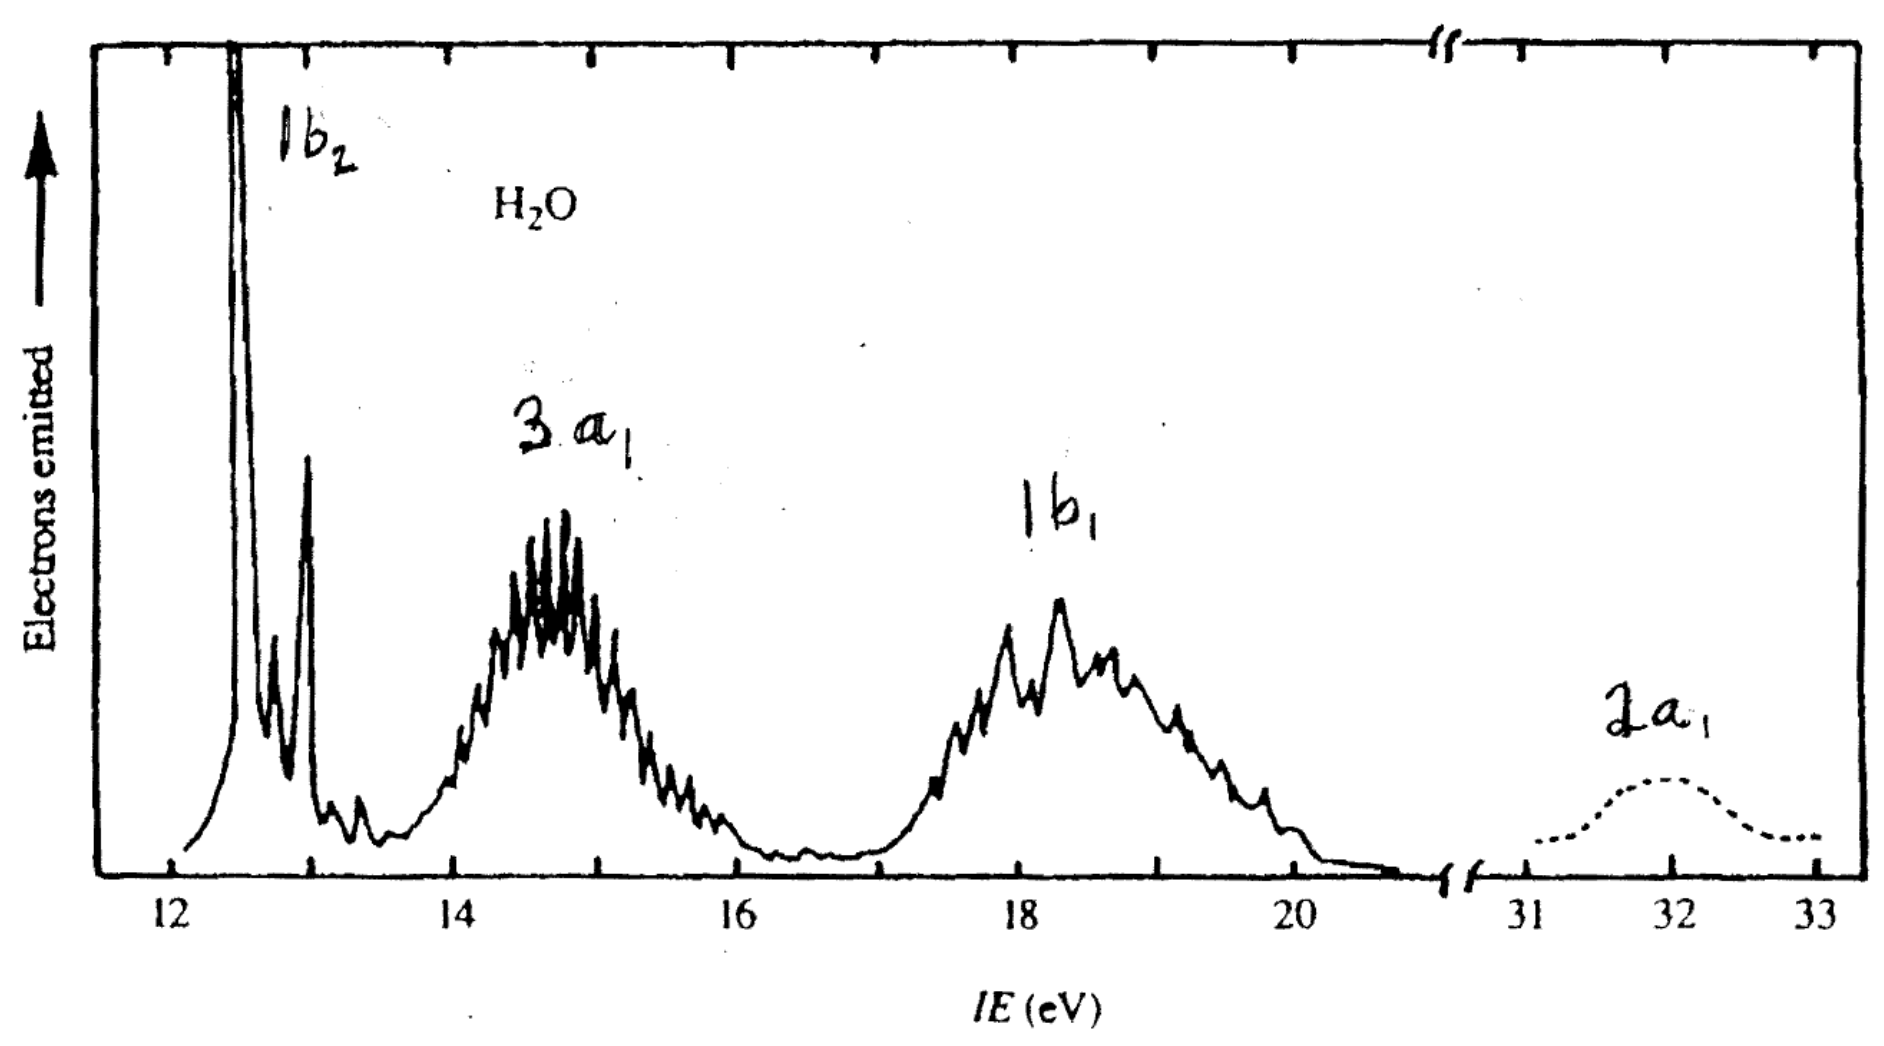
\includegraphics[width=0.6\linewidth]{../ExtFiles/PES-H2O.png}
            \caption{Photoelectron spectrum for \ce{H2O}.}
            \label{fig:PES-H2O}
        \end{figure}
        \begin{itemize}
            \item We see four different states, which matches the prediction of Figure \ref{fig:orbitalDiagram-H2O}.
            \item The lowest state is called $2a_1$ because it is the second state that transforms as $A_1$ going out from the core (the first is $1a_1$ corresponding to oxygen's $1s$ electrons [this state is not shown in Figure \ref{fig:orbitalDiagram-H2O} because it is so core as to not be significantly relevant to the chemistry of \ce{H2O}]).
            \item Then $1b_1$ is the first $B_1$ state going out from the core, $3a_1$ is the third $A_1$ state, and $1b_2$ is the first $B_2$ state.
            \item There are no $4a_1$ and $2b_1$ electrons (see Figure \ref{fig:orbitalDiagram-H2O}); hence, there are no such PES peaks (see Figure \ref{fig:PES-H2O}).
            \item Note that the numbers along the bottom axis correspond to the orbital potential energies of the corresponding molecular orbitals.
        \end{itemize}
        \item For \ce{H2O}, hybridization is qualitatively wrong.
    \end{itemize}
    \item To generate SALCs:
    \begin{itemize}
        \item Use the projection operator. See Nocera Lecture 6 for how to mathematically apply it.
        \item Projection operators constitute a method of generating the symmetry allowed combinations.
        \item Taking one AO and projecting it out using symmetry.
    \end{itemize}
    \item Using the projection operator method to reconstruct SALC orbitals (\ce{NH3} example):
    \begin{figure}[H]
        \centering
        \begin{tikzpicture}
            \footnotesize
            \node (N) {\ce{N}};
            \node (Ha) [circle,draw,inner sep=5pt,label={120:\ce{H_{$a$}}}] at (90:1.5) {}
                edge (N)
            ;
            \node (Hb) [circle,draw,inner sep=5pt,label={-170:\ce{H_{$b$}}}] at (-150:1.5) {}
                edge (N)
            ;
            \node (Hc) [circle,draw,inner sep=5pt,label={-10:\ce{H_{$c$}}}] at (-30:1.5) {}
                edge (N)
            ;
    
            \node (va) at (-90:1.6) {$\sigma_{v(a)}$}
                edge [dashed] (N)
            ;
            \node (vb) at (30:1.6) {$\sigma_{v(b)}$}
                edge [dashed] (N)
            ;
            \node (vc) at (150:1.6) {$\sigma_{v(c)}$}
                edge [dashed] (N)
            ;
    
            \draw [-latex] (N) -- ++(1.9,0) node[below]{$x$};
            \draw [-latex] ([yshift=1mm]Ha.north) -- ++(0,1.3) node[right]{$y$};
    
            \draw [semithick,grx,-latex] (-20:0.6) arc (-20:80:0.6cm);
            \draw [semithick,grx,-latex] (100:0.6) arc (100:200:0.6cm);
            \draw [semithick,grx,-latex] (-140:0.6) arc (-140:-40:0.6cm);
        \end{tikzpicture}
        \caption{Coordinate system for \ce{NH3}.}
        \label{fig:coordinates-NH3}
    \end{figure}
    \begin{table}[h!]
        \centering
        \small
        \renewcommand{\arraystretch}{1.2}
        \begin{tabular}{l|ccc|l|l}
            $C_{3v}$ & $E$ & $2C_3$ & $3\sigma_v$ & linear & quadratic\\
            \hline
            $A_1$ & $1$ & $1$ & $1$ & $z$ & $x^2+y^2,z^2$\\
            $A_2$ & $1$ & $1$ & $-1$ & $R_z$ & \\
            $E$ & $2$ & $-1$ & $0$ & $(x,y),(R_x,R_y)$ & $(x^2-y^2,xy),(xz,yz)$\\
        \end{tabular}
        \caption{Character table for the $C_{3v}$ point group.}
        \label{tab:characterTable-C3v}
    \end{table}
    \begin{itemize}
        \item Ungroup the operations in the classes in Table \ref{tab:characterTable-C3v}. Choose \ce{H_{$a$}} and see into which \ce{H} it projects under each operation. If we order the operations $E,C_3,{C_3}^2,\sigma_{v(a)},\sigma_{v(b)},\sigma_{v(c)}$, then \ce{H_{$a$}} becomes \ce{H_{$a$}}, \ce{H_{$b$}}, \ce{H_{$c$}}, \ce{H_{$a$}}, \ce{H_{$c$}}, \ce{H_{$b$}}, respectively.
        \item Multiply each projected atom by the corresponding character and sum. Thus, for the three representations, we have
        \begin{align*}
            A_1 &= \ce{H_{$a$}}+\ce{H_{$b$}}+\ce{H_{$c$}}+\ce{H_{$a$}}+\ce{H_{$c$}}+\ce{H_{$b$}} = 2\ce{H_{$a$}}+2\ce{H_{$b$}}+2\ce{H_{$c$}}\\
            A_2 &= \ce{H_{$a$}}+\ce{H_{$b$}}+\ce{H_{$c$}}-\ce{H_{$a$}}-\ce{H_{$c$}}-\ce{H_{$b$}} = 0\\
            E &= 2\ce{H_{$a$}}-\ce{H_{$b$}}-\ce{H_{$c$}}+0+0+0 = 2\ce{H_{$a$}}-\ce{H_{$b$}}-\ce{H_{$c$}}
        \end{align*}
        \begin{itemize}
            \item We have essentially just done what the projection operator would enable us to do.
        \end{itemize}
    \end{itemize}
    \item Continuing with the \ce{H2O} example:
    \begin{itemize}
        \item Using the projection operator, we get
        \begin{align*}
            P^{A_1} &= \frac{1}{4}[1E\phi_1+1C_2\phi_1+1\sigma_{xz}\phi_1+1\sigma_{yz}\phi_1] = \frac{1}{2}(\phi_1+\phi_2)\\
            P^{B_1} &= \frac{1}{4}[1E\phi_1-1C_2\phi_1+1\sigma_{xz}\phi_1-1\sigma_{yz}\phi_1] = \frac{1}{2}(\phi_1-\phi_2)
        \end{align*}
        \begin{itemize}
            \item $P^{A_1}$ is a sum of the two hydrogen $1s$ orbitals.
            \item $P^{B_1}$ is a difference of the two hydrogen $1s$ orbitals.
            \item This step allows us to construct electron density maps for the SALCs of the hydrogen's atomic orbitals.
        \end{itemize}
        \item We can now see if the symmetry of various orbitals matches up or doesn't match up and use this information to sketch molecular orbitals.
        \item Oxygen atomic orbital coefficients can only be analytically derived with quantum mechanical calculations.
    \end{itemize}
    \item How can we predict the shape of molecules from MO theory (i.e., without VSEPR theory)?
    \item \textbf{Walsh diagrams} help understand the molecular shapes (bond angles).
    \begin{itemize}
        \item If \ce{H2O} is linear, it is part of the $D_{\infty h}$ point group (which can be reduced to $D_{2h}$ for further mysterious reasons).
        \item $1\sigma_g^+$: If we slowly decrease the bond angle, the hydrogen orbital overlap will increase, meaning that $1\sigma_g^+$ energy decreases.
        \item $1\sigma_u^+$: If we slowly decrease the bond angle, the $s$ and $p$ orbitals will become less aligned, meaning that $1\sigma_u^+$ energy increases.
        \item $\pi_u$, $2a_1$: Energy decreases as hydrogen orbitals get closer to the appropriately signed region of the \ce{O_{$p$}} orbital.
        \item $\pi_u$, $b_2$: Energy is constant.
        \item Now all orbitals with electrons have been accounted for. Since 2 energies go down, 1 goes up, and 1 stays the same as bond angle decreases, we know that bond angle will decrease to an equilibrium.
    \end{itemize}
\end{itemize}



\section{Module 17: Constructing Molecular Orbitals (Part 4, \ce{NH3} Molecule)}
\begin{itemize}
    \item \marginnote{2/3:}\ce{NH3} example:
    \begin{itemize}
        \item Point group: $C_{3v}$.
        \item Basis functions: \ce{H_{$1s$}}, \ce{N_{$2s$}}, \ce{N_{$2p_x$}}, \ce{N_{$2p_y$}}, and \ce{N_{$2p_z$}}.
        \item Apply operations (pick any one operation from each class)/construct reducible representations:
        \begin{align*}
            \Gamma_{\ce{H}} &= (3,0,1) = A_1+E\\
            \Gamma_{\ce{N_{$2s$}}} &= A_1\\
            \Gamma_{\ce{N_{$2p_x$}}} &= E\\
            \Gamma_{\ce{N_{$2p_y$}}} &= E\\
            \Gamma_{\ce{N_{$2p_z$}}} &= A_1
        \end{align*}
        \begin{itemize}
            \item \ce{N_{$2p_x$}} and \ce{N_{$2p_y$}} are doubly degenerate --- their transformation cannot be decoupled and they transform together.
        \end{itemize}
        \item Look at the relevant energies and plot them against each other.
        \item 3 $A_1$ type atomic orbitals form 3 $a_1$ type MOs.
        \begin{figure}[H]
            \centering
            \begin{tikzpicture}[
                yscale=0.2,
                every node/.prefix style={black}
            ]
                \footnotesize
                \draw [ultra thick,gry] (2,-25.56) -- node{\Large$\upharpoonleft$\hspace{-1mm}$\downharpoonright$} node[below=2mm]{$2s(A_1)$} ++(0.5,0);
                \draw [ultra thick,gry]
                    (2,-13.18) -- node{\Large$\upharpoonleft$} node[below=2mm]{$p_x(E)$} ++(0.5,0)
                    ++(0.1,0) -- node{\Large$\upharpoonleft$} node[below=7mm]{$p_y(E)$} ++(0.5,0)
                    ++(0.1,0) -- node{\Large$\upharpoonleft$} node[below=2mm]{$p_z(A_1)$} ++(0.5,0)
                ;
                \draw [ultra thick,gry]
                    (-3.7,-13.61) -- node{\Large$\upharpoonleft$} node[below=2mm]{$A_1$} ++(0.5,0)
                    ++(0.1,0) -- node{\Large$\upharpoonleft$} node[below=2mm]{$E$} ++(0.5,0)
                    ++(0.1,0) -- node{\Large$\upharpoonleft$} node[below=2mm]{$E$} ++(0.5,0)
                ;
        
                \draw [ultra thick] (-0.55,-35) -- node{\Large$\upharpoonleft$\hspace{-1mm}$\downharpoonright$} node[below=2mm]{$2a_1$} ++(1.1,0);
                \draw [ultra thick] (-0.55,-26) -- node{\Large$\upharpoonleft$\hspace{-1mm}$\downharpoonright$} ++(0.5,0) node[below=2mm,xshift=0.05cm]{$1e$} ++(0.1,0) -- node{\Large$\upharpoonleft$\hspace{-1mm}$\downharpoonright$} ++(0.5,0);
                \draw [ultra thick] (-0.55,-19) -- node{\Large$\upharpoonleft$\hspace{-1mm}$\downharpoonright$} node[below=2mm]{$3a_1$} ++(1.1,0);
                \draw [ultra thick] (-0.55,-9) -- ++(0.5,0) node[below,xshift=0.05cm]{$2e$} ++(0.1,0) -- ++(0.5,0);
                \draw [ultra thick] (-0.55,-5) -- node[below]{$4a_1$} ++(1.1,0);
        
                \draw [grx,densely dashed]
                    (-3.2,-13.61) -- (-0.55,-35)
                    (-3.2,-13.61) -- (-0.55,-19)
                    (-3.2,-13.61) -- (-0.55,-5)
                    (-2,-13.61) -- (-0.55,-26)
                    (-2,-13.61) -- (-0.55,-9)
                    (2,-13.18) -- (0.55,-9)
                    (2,-13.18) -- (0.55,-26)
                    (3.2,-13.18) -- (0.55,-5)
                    (3.2,-13.18) -- (0.55,-19)
                    (2,-25.56) -- (0.55,-19)
                    (2,-25.56) -- (0.55,-35)
                ;
            \end{tikzpicture}
            \caption{\ce{NH3} orbital diagram.}
            \label{fig:orbitalDiagram-NH3}
        \end{figure}
        \begin{itemize}
            \item Since $2s(A_1)$ and $1s(A_1)$ are so far away energetically, their combination will have very low energy.
            \item On the other hand, since the $2s(A_1)$ and $p_z(A_1)$ are close in energy, they have a lot of overlap.
            \item We can't analytically calculate orbital energies at this level. Take an educated guess on the homework and explain your reasoning. Note that here, $e$ orbitals are more stabilizing because they are bigger and have larger overlap. Also, $\sigma$ bonds are stronger than $\pi$ bonds because there is a higher degree of overlap.
        \end{itemize}
        \item To see what these orbitals look like, we need to apply the projection operator.
        \begin{itemize}
            \item We need to construct one $A_1$ orbital and two $E$ orbitals.
            \item Modifying from the example from last time, we have $P^{A_1}\approx\phi_1+\phi_2+\phi_3$ and $P^E\approx 2\phi_1-\phi_2-\phi_3$.
            \item For the last $E$ SALC, we apply the projection to each hydrogen atom (we can choose any basis function) giving us, in addition to the other projections, $P^E\approx 2\phi_2-\phi_3-\phi_1$ and $P^E\approx 2\phi_3-\phi_1-\phi_2$. By subtracting these two, we get $\Psi_E=\frac{1}{\sqrt{2}}(\phi_2-\phi_3)$. Do we choose this linear combination because it's orthogonal to the other two? Because it's structure is different and simple (you \emph{can} do it with any linear combination, but it will make the analysis much more complicated if you do it with a trickier linear combination).
        \end{itemize}
        \item We need to renormalize our SALCs so that the integral of their square over all space is 1. To normalize, we must guarantee that the sum of the squares of the coefficients is 1. For $P^{A_1}$ for example, $1^2+1^2+1^2=3$, so we must scale the whole thing by $\frac{1}{\sqrt{3}}$.
        \item In the PES spectrum, we see three peaks, one being approximately twice as wide as the others (corresponding to the double degenerate state).
        \item Walsh diagrams (rely on the pictures that we draw of orbitals):
        \begin{itemize}
            \item $1a_1'$ energy decreases, $1e'$ energy increases, $a_2''$ energy decreases rather dramatically.
            \item If we promote electrons to the excited state, the relevant Walsh diagrams will change, and this will cause the molecule to change shape.
        \end{itemize}
    \end{itemize}
    \item Also try to sketch the MOs in the homework.
\end{itemize}



\section{Module 18: Constructing Molecular Orbitals (Part 5, \ce{H2C=CH2} Molecule)}
\begin{itemize}
    \item \ce{H2C=CH2} example:
    \begin{figure}[h!]
        \centering
        \begin{subfigure}[b]{0.49\linewidth}
            \centering
            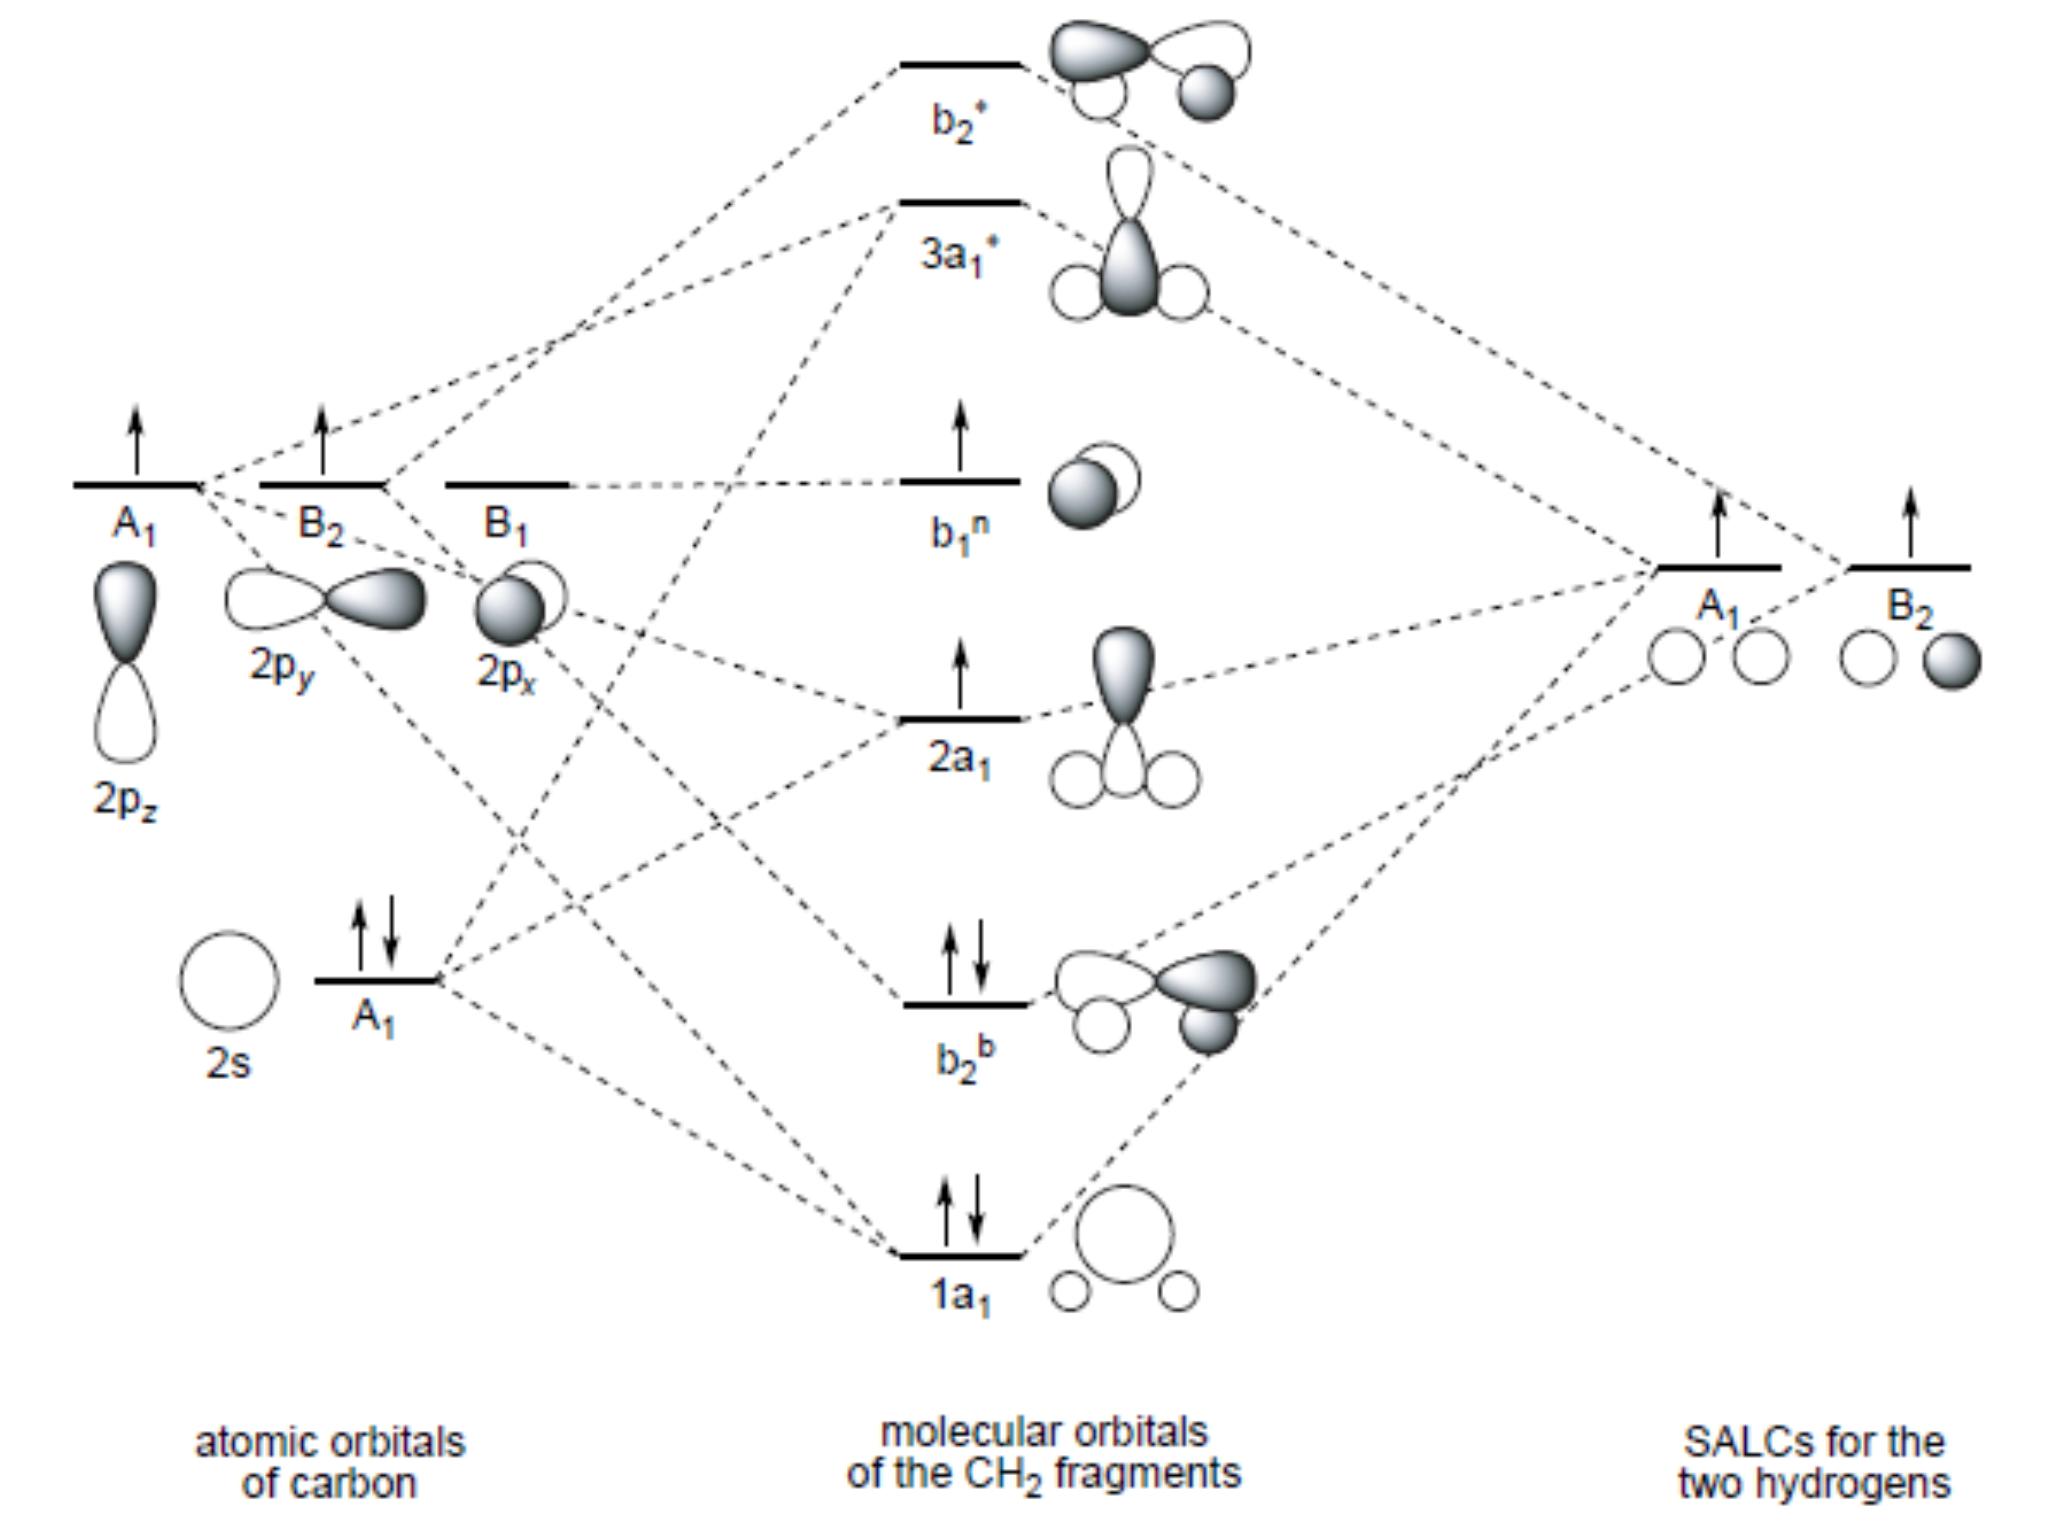
\includegraphics[width=0.9\linewidth]{../ExtFiles/orbitalDiagram-C2H4a.png}
            \caption{Carbene fragment.}
            \label{fig:orbitalDiagram-C2H4a}
        \end{subfigure}
        \begin{subfigure}[b]{0.49\linewidth}
            \centering
            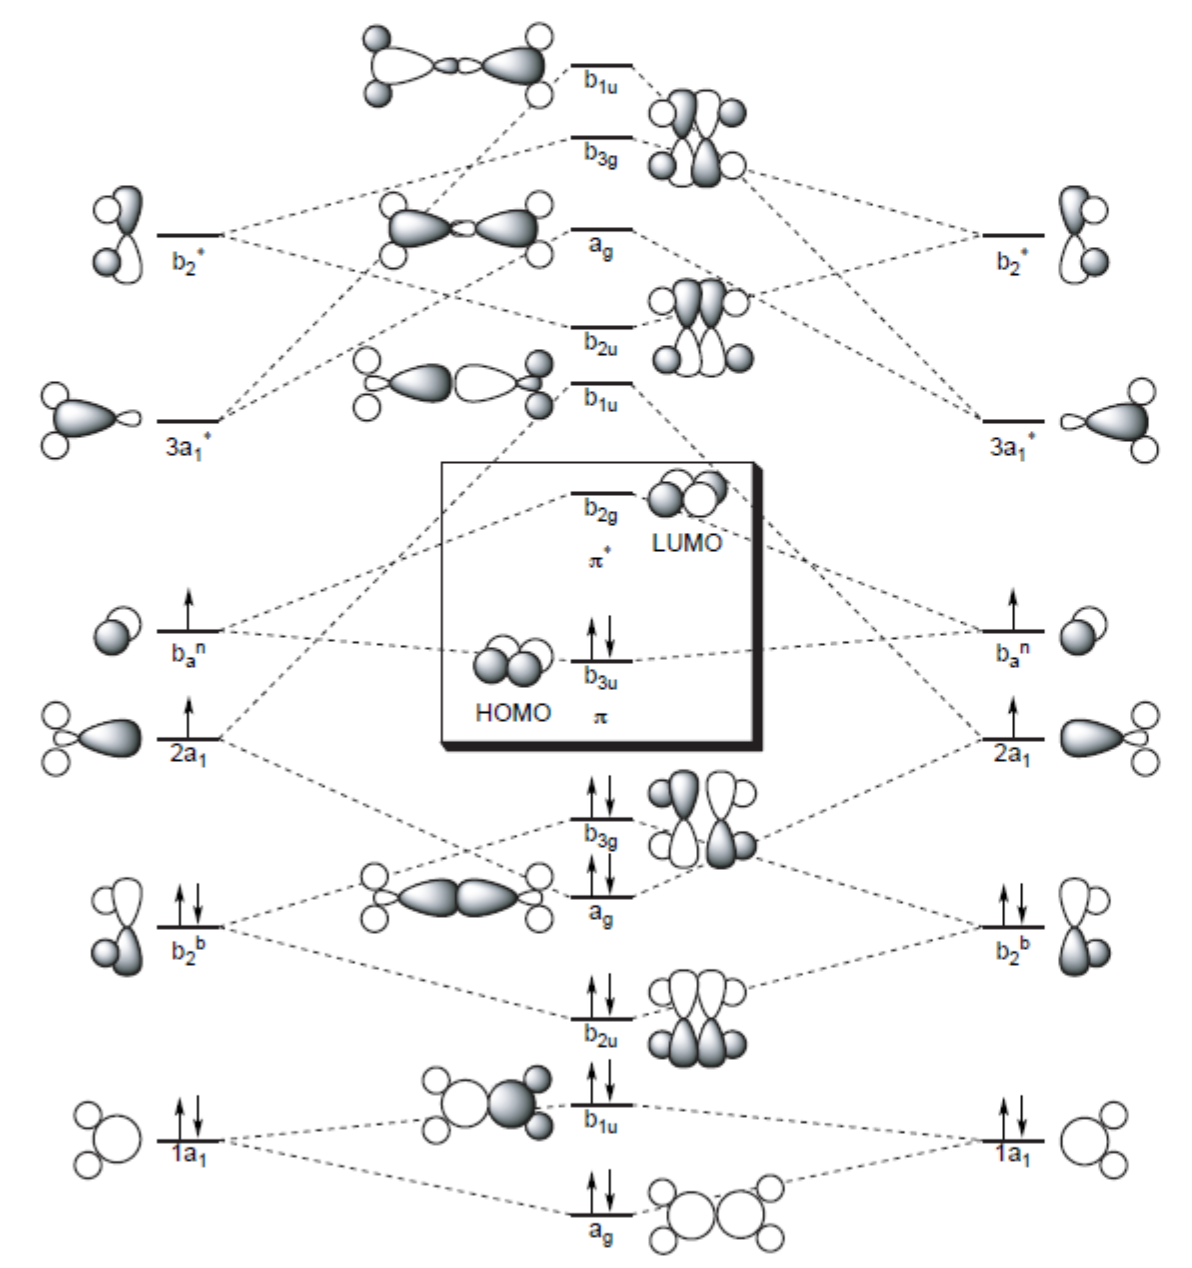
\includegraphics[width=0.7\linewidth]{../ExtFiles/orbitalDiagram-C2H4b.png}
            \caption{Full molecule.}
            \label{fig:orbitalDiagram-C2H4b}
        \end{subfigure}
        \caption{\ce{H2C=CH2} orbital diagram.}
        \label{fig:orbitalDiagram-C2H4}
    \end{figure}
    \begin{itemize}
        \item Two different approaches ($D_{2h}$): \ce{C_1 + C_2} then \ce{H_{1-4}}, or two carbene fragments (\ce{CH2}).
        \begin{itemize}
            \item We can read about the first approach in the linked JCE article \parencite{bib:reinforceMOTheory}.
        \end{itemize}
        \item $C_{2v}$ for the \ce{CH2} fragment.
        \item When we make the MO diagram, we have two unpaired electrons, one in each of the upper two orbitals. These will be used for bonding to the other carbene fragment.
        \item We will then combine the MO diagrams and will need to reassign orbital names because ethene isn't $C_{2v}$; it's $D_{2h}$.
    \end{itemize}
\end{itemize}



\section{Module 19: Isolobal Principle}
\begin{itemize}
    \item \textbf{Isolobal} (fragment): A fragment with similar (not identical) numbers, symmmetry properties, approximate energies, and shapes of the frontier orbitals and the number of electrons in them.
    \item This allows us to show, for example, that a carbene fragment and a $d^7$ metal complex have similar properties.
    \item Two \ce{CH3} fragments will tend to couple into ethane. But so will two isolobal \ce{Mn(CO)5} fragments!
\end{itemize}



\section{Module 20: Orbital Hybridization}
\begin{itemize}
    \item \textbf{Hybridization}: The concept of mixing atomic orbitals into new hybrid orbitals (with different energies, shapes, etc. than the component atomic orbitals) suitable for the pairing of electrons to form chemical bonds.
    \item Hybridization accomplishes the work of MO theory in steps: Creating new orbitals and then bonding atoms with them, as opposed to defining new orbitals and filling them.
    \item This was the dominant approach in chemistry before MO theory, and is still widely used in organic chemistry.
    \item For light elements, the energy gaps between orbitals aren't very large and this method is legitimate to some degree.
    \begin{itemize}
        \item For carbon, it's acceptable.
        \item For silicon and lead (in the same group), this is not a good approach; it will give you incorrect predictions (e.g., around bond angles and lengths).
    \end{itemize}
    \item Steps to determine the hybridization of a bond:
    \begin{enumerate}
        \item Assign a point group.
        \item Choose basis function ($\sigma$ bonds).
        \item Apply operations.
        \item Reduce to irreducible representations.
        \item Compare symmetry of irreducible representations to central atom MOs.
    \end{enumerate}
    \item \ce{BF3} example:
    \begin{itemize}
        \item Point group: $D_{3h}$.
        \item $\Gamma_\sigma=(3,0,1,3,0,1)$.
        \item $\Gamma_\sigma=A_1'+E'$.
        \item For boron, $\ce{B}(s)=A_1'$, $\ce{B}(p_x)=E'$, $\ce{B}(p_y)=E'$, and $\ce{B}(p_z)=A_2''$. Thus, since one orbital matches up on $s$ and two match up on $p$ (specifically, $p_x,p_y$), the hybrid orbitals will be $sp^2$ (hybrid of $s,p_x,p_y$).
    \end{itemize}
    \item It is not generally justifiable to say that atomic orbitals in \emph{individual} atoms mix before bonding.
\end{itemize}



\section{Chapter 5: Molecular Orbitals}
\emph{From \textcite{bib:MiesslerFischerTarr}.}
\begin{itemize}
    \item \marginnote{1/29:}MO theory uses group theory to describe molecular bonding, complementing and extending Chapter 3.
    \item "In molecular orbital theory the symmetry properties and relative energies of atomic orbitals determine how these orbitals interact to form molecular orbitals" \parencite[117]{bib:MiesslerFischerTarr}.
    \item The molecular orbitals are filled according to the same rules discussed in Chapter 2.
    \item If the total energy of the electrons in the molecular orbitals is less than that of them in the atomic orbitals, the molecule is stable relative to the separate atoms (and forms). If the total energy of the electrons in the molecular orbitals exceeds that of them in the atomic orbitals, the molecule is unstable (and does not form).
    \item \textbf{Homonuclear} (molecule): A molecule in which all constituent atoms have the same atomic number.
    \item \textbf{Heteronuclear} (molecule): A molecule that is not homonuclear, i.e., one in which at least two atoms differ in atomic number.
    \item A less rigorous pictorial approach can describe bonding in many small molecules and help us to build a more rigorous one, based on symmetry and employing group theory, that will be needed to understand orbital interactions in more complex molecular structures.
    \item Schr\"{o}dinger equations can be written for electrons in molecules as they can for electrons in atoms. Approximate solutions can be constructed from the LCAO method.
    \begin{itemize}
        \item In diatomic molecules for example, $\Psi=c_a\psi_a+c_b\psi_b$ where $\Psi$ is the molecular wave function, $\psi_{a,b}$ are the atomic wave functions for atoms $a$ and $b$, and $c_{a,b}$ are adjustable coefficients that quantify the contribution of each atomic orbital to the molecular orbital.
    \end{itemize}
    \item "As the distance between two atoms is decreased, their orbitals overlap, with significant probability for electrons from both atoms being found in the region of overlap" \parencite[117]{bib:MiesslerFischerTarr}.
    \item Electrostatic forces between nuclei and electrons in bonding molecular orbitals hold atoms together.
    \item \marginnote{2/5:}Precise calculations show that the coefficient of the $\sigma^*$ hydrogen antibonding orbital is slightly larger than that of the $\sigma$ orbital, but we typically neglect this distinction.
    \begin{itemize}
        \item This technically implies that $\Delta E_{\sigma^*}>\Delta E_\sigma$, i.e., that the increase in energy from electrons in atomic orbitals moving into the $\sigma^*$ antibonding molecular orbital is greater in magnitude than the decrease in energy from electrons in atomic orbitals moving into the $\sigma$ bonding molecular orbital.
    \end{itemize}
    \item \textbf{$\bm{\sigma}$ orbital}: A molecular orbital that is symmetric to rotation about the line connecting the nuclei.
    \item \textbf{Orbital asterisk}: Denotes antibonding orbitals for those molecules where bonding and antibonding orbital descriptions are unambiguous (i.e., smaller molecules).
    \item When two regions of like sign overlap, the sum of the orbitals exhibits increased electron probability in the overlap region, and vice versa for regions of opposite sign.
    \item When the $z$-axes are drawn pointing in the same direction, their difference is $\sigma$ and their sum is $\sigma^*$.
    \begin{figure}[h!]
        \centering
        \begin{subfigure}[b]{0.4\linewidth}
            \centering
            \begin{tikzpicture}
                \begin{scope}[xshift=-1.2cm]
                    \filldraw [draw=black,fill=grt] (0,0)
                        to[out=90,in=90,out looseness=0.5] (0.8,0)
                        to[out=-90,in=-90,in looseness=0.5] cycle
                    ;
                    \draw [rotate=180] (0,0)
                        to[out=90,in=90,out looseness=0.5] (0.8,0)
                        to[out=-90,in=-90,in looseness=0.5] cycle
                    ;
                    \draw [->] (-1,0) -- (1,0);
                \end{scope}
                \begin{scope}[xshift=1.2cm]
                    \filldraw [draw=black,fill=grt] (0,0)
                        to[out=90,in=90,out looseness=0.5] (0.8,0)
                        to[out=-90,in=-90,in looseness=0.5] cycle
                    ;
                    \draw [rotate=180] (0,0)
                        to[out=90,in=90,out looseness=0.5] (0.8,0)
                        to[out=-90,in=-90,in looseness=0.5] cycle
                    ;
                    \draw [->] (-1,0) -- (1,0);
                \end{scope}
            \end{tikzpicture}
            \caption{Same direction.}
            \label{fig:z-axisDirectiona}
        \end{subfigure}
        \begin{subfigure}[b]{0.4\linewidth}
            \centering
            \begin{tikzpicture}
                \begin{scope}[xshift=-1.2cm]
                    \filldraw [draw=black,fill=grt] (0,0)
                        to[out=90,in=90,out looseness=0.5] (0.8,0)
                        to[out=-90,in=-90,in looseness=0.5] cycle
                    ;
                    \draw [rotate=180] (0,0)
                        to[out=90,in=90,out looseness=0.5] (0.8,0)
                        to[out=-90,in=-90,in looseness=0.5] cycle
                    ;
                    \draw [->] (-1,0) -- (1,0);
                \end{scope}
                \begin{scope}[xshift=1.2cm,rotate=180]
                    \filldraw [draw=black,fill=grt] (0,0)
                        to[out=90,in=90,out looseness=0.5] (0.8,0)
                        to[out=-90,in=-90,in looseness=0.5] cycle
                    ;
                    \draw [rotate=180] (0,0)
                        to[out=90,in=90,out looseness=0.5] (0.8,0)
                        to[out=-90,in=-90,in looseness=0.5] cycle
                    ;
                    \draw [->] (-1,0) -- (1,0);
                \end{scope}
            \end{tikzpicture}
            \caption{Opposite directions.}
            \label{fig:z-axisDirectionb}
        \end{subfigure}
        \caption{Choice of $z$-axis direction.}
        \label{fig:z-axisDirection}
    \end{figure}
    \begin{itemize}
        \item Notice how in Figure \ref{fig:z-axisDirectionb}, we can simply push the orbitals together (add them) to have regions of like sign overlap and form a bonding orbital.
        \item However, in Figure \ref{fig:z-axisDirectiona}, with a more standard coordinate system, we have to flip the signs of one of the orbitals before merging them (multiply it by $-1$ and add it to the other orbital/subtract it from the other orbital) to create a bonding orbital. If we add them as they are, we will get an antibonding orbital.
    \end{itemize}
    \item \textbf{$\bm{\pi}$ orbital}: A molecular orbital with a change in sign of the wave function under $C_2$ rotation about the $z$-axis (the bond axis).
    \begin{itemize}
        \item $\pi$ and $\pi^*$ orbitals arise from the interactions between $p_x$ and $p_y$ atomic orbitals.
    \end{itemize}
    \item MOs that form from $p_z$ orbitals are $\sigma$ and $\sigma^*$ orbitals.
    \item "When orbitals overlap equally with both the same and opposite signs\dots the bonding and antibonding effects cancel, and no molecular orbital results" \parencite[121]{bib:MiesslerFischerTarr}.
    \item $d$ orbitals can also be involved in bonding in heavier elements such as the transition metals.
    \begin{itemize}
        \item Two $d_{z^2}$ orbitals participate in $\sigma$ bonding.
        \item Two $d_{xz}$ or $d_{yz}$ orbitals participate in $\pi$ bonding.
        \item Two $d_{x^2-y^2}$ or $d_{xz}$ orbitals participate in \textbf{$\bm{\delta}$ bonding}.
    \end{itemize}
    \item \textbf{$\bm{\delta}$ orbital}: A molecular orbital with a change in sign of the wave function under $C_4$ rotation about that $z$-axis.
    \begin{itemize}
        \item $\delta$ and $\delta^*$ orbitals arise from the interactions of atomic orbitals meeting in parallel planes and combining side to side.
    \end{itemize}
    \item "Sigma orbitals have no nodes that include the line connecting the nuclei, pi orbitals have one node that includes the line connecting the nuclei, and delta orbitals have two nodes that include the line connecting the nuclei" \parencite[121]{bib:MiesslerFischerTarr}.
    \item Note that $p_x$ and $d_{xz}$ orbitals (for example) could, in theory, interact.
    \item Additional thoughts on Figure \ref{fig:orbitalEnergyCombinations}:
    \begin{itemize}
        \item Similarity in energy is correlated with similarity in structure.
        \item When orbital energies are similar (Figure \ref{fig:orbitalEnergyCombinationsa}), there is a large difference between the atomic orbitals and the molecular orbitals, resulting in a great potential for stabilization through bonding.
    \end{itemize}
    \item Molecular orbitals help us understand the structure of \ce{Li2}, \ce{Be2}, and other diatomic molecules that violate the octet rule.
    \begin{itemize}
        \item They also explain experimental phenomena that clash with VSEPR theory --- for example, the Lewis structure of \ce{O2} predicts a diamagnetic molecule, but in reality, \ce{O2} is paramagnetic with two unpaired electrons.
    \end{itemize}
    \item See Figure \ref{fig:molecularOrbitals-first10} for the molecular orbitals in the homonuclear diatomic molecules formed by the first 10 elements, neglecting interactions between atomic orbitals of differing energy levels.
    \begin{figure}[h!]
        \centering
        \begin{tikzpicture}
            \footnotesize
            \draw [white] (-6,0) -- (6,0);
            \node at (4,6.3) {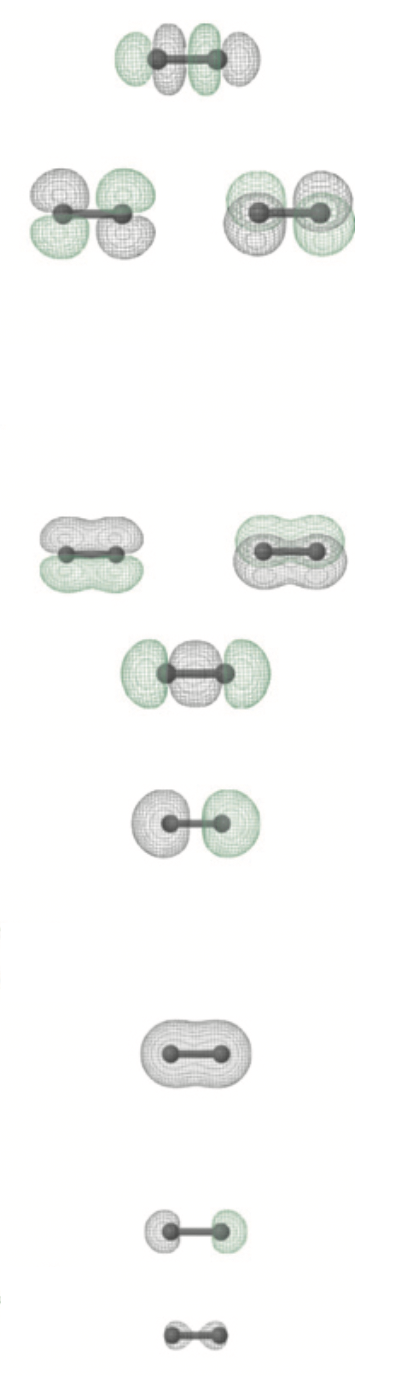
\includegraphics[width=0.24\linewidth]{../ExtFiles/molecularOrbitals-first10.png}};
    
            \draw [ultra thick]
                (-2.4,0) -- node[above]{$1s$} ++(0.4,0) coordinate (1sl)
                (2,0) coordinate (1sr) -- node[above]{$1s$} ++(0.4,0)
                (-2.4,3) -- node[above]{$2s$} ++(0.4,0) coordinate (2sl)
                (2,3) coordinate (2sr) -- node[above]{$2s$} ++(0.4,0)
                (-3.4,9) -- ++(0.4,0) ++(0.1,0) -- node[above]{$2p$} ++(0.4,0) ++(0.1,0) -- ++(0.4,0) coordinate (2pl)
                (2,9) coordinate (2pr) -- ++(0.4,0) ++(0.1,0) -- node[above]{$2p$} ++(0.4,0) ++(0.1,0) -- ++(0.4,0)
            ;
            \draw [ultra thick]
                (-0.25,-0.1) coordinate (og1l) -- node[below]{$\sigma_g$}   ++(0.5,0) coordinate (og1r)
                (-0.25,0.2)  coordinate (ou1l) -- node[above]{$\sigma_u^*$} ++(0.5,0) coordinate (ou1r)
                (-0.25,2)    coordinate (og2l) -- node[above]{$\sigma_g$}   ++(0.5,0) coordinate (og2r)
                (-0.25,4.3)  coordinate (ou2l) -- node[above]{$\sigma_u^*$} ++(0.5,0) coordinate (ou2r)
                (-0.25,6)    coordinate (og3l) -- node[above]{$\sigma_g$}   ++(0.5,0) coordinate (og3r)
                (-0.25,12.5) coordinate (ou3l) -- node[above]{$\sigma_u^*$} ++(0.5,0) coordinate (ou3r)
                (-0.55,7) coordinate (pul) -- node[above]{$\pi_u$} ++(0.5,0) ++(0.1,0) -- node[above]{$\pi_u$} ++(0.5,0) coordinate (pur)
                (-0.55,11) coordinate (pgl) -- node[above]{$\pi_g^*$} ++(0.5,0) ++(0.1,0) -- node[above]{$\pi_g^*$} ++(0.5,0) coordinate (pgr)
            ;
    
            \draw [thick,grx,densely dashed]
                (1sl) -- (og1l)
                (1sr) -- (og1r)
                (1sl) -- (ou1l)
                (1sr) -- (ou1r)
                (2sl) -- (og2l)
                (2sr) -- (og2r)
                (2sl) -- (ou2l)
                (2sr) -- (ou2r)
                (2pl) -- (og3l)
                (2pr) -- (og3r)
                (2pl) -- (ou3l)
                (2pr) -- (ou3r)
                (2pl) -- (pul)
                (2pr) -- (pur)
                (2pl) -- (pgl)
                (2pr) -- (pgr)
            ;
    
    
            \draw [semithick]
                (-3.5,-0.4) ellipse (8mm and 4mm)
                (-4,0.4) circle (2.5mm)
            ;
            \filldraw [semithick,draw,fill=grt] (-3,0.4) circle (2.5mm);
            \fill
                (-4,-0.4) circle (1pt)
                (-3,-0.4) circle (1pt)
                (-4,0.4) circle (1pt)
                (-3,0.4) circle (1pt)
            ;
    
            \draw [semithick]
                (-3.5,2) ellipse (8mm and 4mm)
                (-4,4.3) circle (2.5mm)
            ;
            \filldraw [semithick,draw,fill=grt] (-3,4.3) circle (2.5mm);
            \fill
                (-4,2) circle (1pt)
                (-3,2) circle (1pt)
                (-4,4.3) circle (1pt)
                (-3,4.3) circle (1pt)
            ;
    
            \draw [semithick]
                (-3.5,6) ellipse (4.7mm and 2.4mm)
                (-2.4,12.5) circle (2.5mm)
                (-3.8,12.5) ellipse (2.5mm and 5mm)
            ;
            \filldraw [semithick,draw,fill=grt]
                (-4.2,6) ellipse (2.4mm and 2.5mm)
                (-2.8,6) ellipse (2.4mm and 2.5mm)
                (-4.6,12.5) circle (2.5mm)
                (-3.2,12.5) ellipse (2.5mm and 5mm)
            ;
            \fill
                (-4.2,12.5) circle (1pt)
                (-2.8,12.5) circle (1pt)
            ;
    
            \draw [semithick]
                (-3.5,7.85) ellipse (8mm and 4mm)
                (-4,11) ellipse (4mm and 2.5mm)
                (-3,10.2) ellipse (4mm and 2.5mm)
            ;
            \filldraw [semithick,draw,fill=grt]
                (-3.5,6.95) ellipse (8mm and 4mm)
                (-3,11) ellipse (4mm and 2.5mm)
                (-4,10.2) ellipse (4mm and 2.5mm)
            ;
            \fill
                (-4,7.4) circle (1pt)
                (-3,7.4) circle (1pt)
                (-4,10.6) circle (1pt)
                (-3,10.6) circle (1pt)
            ;
        \end{tikzpicture}
        \caption{Molecular orbitals for the first 10 elements.}
        \label{fig:molecularOrbitals-first10}
    \end{figure}
    \item Bond order:
    \begin{equation*}
        \text{B.O.} = \frac{1}{2}(\text{number of electrons in bonding orbitals}-\text{number of electrons in antibonding orbitals})
    \end{equation*}
    \begin{itemize}
        \item Generally, we need only consider valence electrons to calculate the bond order: For example, \ce{O2} has $\text{B.O.}=2$ whether or not you factor valence electrons into the calculation.
    \end{itemize}
    \item Core electrons are generally assumed to reside mostly on the original atom and negligibly participate in bonding and antibonding interactions.
    \begin{itemize}
        \item This is reflected by how much lower the $1s$ MOs are in Figure \ref{fig:molecularOrbitals-first10} than the others, and by how slight the difference is between bonding and antibonding.
    \end{itemize}
    \item "When two molecular orbitals of the same symmetry have similar energies, they interact to lower the energy of the lower orbital and raise the energy of the higher orbital" \parencite[124]{bib:MiesslerFischerTarr}.
    \item \textbf{$\bm{\sigma_g}$ symmetry}: Symmetry to infinite rotation and inversion.
    \begin{itemize}
        \item Possessed by the $\sigma_g(2s)$ and $\sigma_g(2p)$ orbitals in Figure \ref{fig:molecularOrbitals-first10}, for example.
    \end{itemize}
    \item Molecular orbitals with the same symmetry and similar energies can \textbf{mix}, lowering the energy of the lower orbital and raising the energy of the higher orbital.
    \begin{itemize}
        \item For example, the $\sigma_g(2s)$ and $\sigma_g(2p)$ orbitals in Figure \ref{fig:molecularOrbitals-first10} can mix, lowering the energy of the $2s$ one and raising the energy of the $2p$ one.
    \end{itemize}
    \item \marginnote{2/6:}Atomic orbital energies decrease across a row in the periodic table.
    \item Characterization of selected homonuclear diatomic molecules:
    \begin{itemize}
        \item \ce{He2}'s bond order is 0, with two bonding and two antibonding electrons. Thus, it has no significant tendency to form (it's bond energy is $\SI[per-mode=symbol]{0.01}{\joule\per\mole}$, compared to \ce{H2}'s $\SI[per-mode=symbol]{436}{\kilo\joule\per\mole}$).
        \item \ce{B2} is paramagnetic (because of its two unpaired $\pi_u$ electrons). The $2p$ valence electrons do not occupy the $\sigma_g$ MO because of orbital mixing and because the energy difference between $\sigma_g(2p)$ and $\pi_u(2p)$ is greater than $\Pi_c$ (even if there were no mixing, the electrons would still occupy the $\pi_u$ orbitals if it was more energetically favorable to do this than to occupy the same orbital).
        \item \ce{C2} is a rarely encountered allotrope of carbon, but it has two $\pi$ bonds and no $\sigma$ bonds.
        \item In \ce{N2}, some larger trends become apparent:
        \begin{itemize}
            \item Since electrons in different orbitals vary in their shielding abilities and electron-electron interactions, the difference between the $2s$ and $2p$ energies increase as $Z$ increases.
            \item More specifically, $2s$ electrons have higher probabilities close to the nucleus than $2p$ electrons (Figure \ref{fig:radialProbability}), so they are more affected by increasing nuclear charge (inverse square law).
            \item As a result of this separation, the $\sigma_g(2s)$ and $\sigma_g(2p)$ orbitals mix less in \ce{N2} than in \ce{C2} or \ce{B2}.
        \end{itemize}
        \item The ions of \ce{O2} (which include dioxygenyl \ce{O2+}, superoxide \ce{O2-}, and peroxide \ce{O2^2-}) reveal that bond order and bond distance are inversely proportional. Here, mixing finally becomes small enough that the normal filling order (as in Figure \ref{fig:molecularOrbitals-first10}) returns.
    \end{itemize}
    \item Notice how atomic radius consistently decreases across the second period, but bond length decreases until \ce{N2} and then increases (because of the addition of antibonding electrons).
    \item At this point, we'll assume (for PES purposes) the energy levels in the uncharged molecule to be essentially the same as those in the charged ions generated when we seek to examine core energy levels\footnote{However, we should note that this is an oversimplification; a rigorous treatment of PES considers how the energy levels and orbital shapes vary between the neutral and ionized species.}.
    \item Comparing the PES spectra for \ce{N2} and \ce{O2}, it can be seen that the \ce{N2} energy levels are closer together than the \ce{O2} ones.
    \item PES also provides evidence for the existence of \textbf{vibrational energy levels}, energy levels that are much more closely spaced than electronic levels that cause the multiple peaks within one "peak."
    \item Orbitals that are strongly involved in bonding have \textbf{vibrational fine structure} (multiple peaks), and vice versa for less involved orbitals.
    \begin{itemize}
        \item Thus, the 10 $\pi_u$ vs. the 6 $\sigma_g$ vibrational peaks in \ce{O2} indicate that the $\pi_u$ orbitals are more strongly involved in bonding than the $\sigma_g$ orbital.
    \end{itemize}
    \item "The atomic orbitals of atoms that form homonuclear diatomic molecules have identical energies, and both atoms contribute equally to a given MO. Therefore, in the molecular orbital equations, the coefficients associated with the same atomic orbitals of each atom\dots are identical. In heteronuclear diatomic molecules\dots the atomic orbitals have different energies, and a given MO receives unequal contributions from these atomic orbitals; the MO equation has a different coefficient for each of the atomic orbitals that contribute to it" \parencite[134,136]{bib:MiesslerFischerTarr}.
    \item Atomic orbitals closer in energy to an MO contribute more to that MO, and thus have larger coefficients in the wave equation.
    \item \ce{CO} example:
    \begin{itemize}
        \item The $1\pi$ orbitals are lower than the $3\sigma$ orbitals because of the strong mixing between the $2p_z$ orbital of oxygen and the $2s$ and $2p_z$ orbitals of carbon.
        \item The $3\sigma$ orbital has a large lobe on the carbon end because two carbon orbitals ($2s$ and $2p_z$) mix with one oxygen orbital ($2p_z$).
        \item The $\pi$ orbital has electron density concentrated on oxygen because of the better energy match between the MO and the $2p_{x,y}$ orbitals of oxygen; the $\pi^*$ orbital has electron density concentrated on carbon because of the better energy match between the MO and the $2p_{x,y}$ orbitals of carbon.
    \end{itemize}
    \item Atomic orbitals with energy differences greater than 10-14 eV usually do not interact significantly.
    \item MOs in \ce{HF} predict a polar bond since electron density is concentrated on \ce{F} to such a greater extent in every occupied orbital.
    \item \textbf{Frontier orbitals}: The HOMO and LUMO, so-named because they lie at the occupied-unoccupied frontier.
    \item Frontier orbitals help explain reaction chemistry with transition metals.
    \begin{itemize}
        \item In \ce{CO} for example, we'd predict based on electronegativity that the \ce{O} would be more reactive, and hence we'd get a preponderance of \ce{M-O-C} structures.
        \item However, carbonyl complexes are typically of the form \ce{M-C-O} because the frontier orbitals both lie more on \ce{C}. Indeed, the HOMO contains the least stabilized (most reactive) electrons in the molecule, and the LUMO is ready to accept whatever electrons are donated first.
    \end{itemize}
    \item Ionic compounds can still be treated, MO theory-wise, like covalent compounds; we just get MOs that are almost identical to the more favored constitutent atomic orbitals.
    \item Crystalline lattice salts are much more stable than diatomic ones.
    \begin{itemize}
        \item Such crystal lattices are held together by a combination of electrostatics (ionic) attraction and covalent bonding.
        \item Salts do not exhibit directional bonds; instead, the orbitals form energy bands (see Chapter 7).
    \end{itemize}
    \item Considers lattice enthalpies and Born-Haber cycles\footnote{See \textcite{bib:APChemNotes}, specifically Figure 8.2 and the associated discussion}.
    \item \textbf{Group orbitals}: Collections of matching orbitals on outer atoms.
    \begin{itemize}
        \item Sets of orbitals that potentially could interact with the central atom orbitals.
        \item The same combinations that formed bonding and antibonding orbitals in diatomics.
    \end{itemize}
    \item \ce{FHF-} example:
    \begin{itemize}
        \item The group orbitals are formed by adding and subtracting the \ce{F} orbitals as we would in \ce{F2}.
        \begin{figure}[h!]
            \centering
            \begin{tikzpicture}
                \footnotesize
                \begin{scope}[xshift=-5cm]
                    \node at (0,2.5) {\underline{Fluorine Orbitals Used}};
                    \node at (0,1.5) {$2p_z$};
                    \node at (0,0) {$2s$};
                \end{scope}
                \begin{scope}
                    \node at (0,2.5) {\underline{Bonding}};
        
                    \draw [semithick]
                        (0,1.5) circle (2.5mm)
                        (-0.6,1.5) ellipse (2.5mm and 5mm)
                        (0.6,1.5) ellipse (2.5mm and 5mm)
                    ;
                    \filldraw [semithick,draw,fill=grt]
                        (-1.4,1.5) ellipse (2.5mm and 5mm)
                        (1.4,1.5) ellipse (2.5mm and 5mm)
                    ;
                    \fill
                        (0,1.5) circle (1pt)
                        (-1,1.5) circle (1pt)
                        (1,1.5) circle (1pt)
                    ;
        
                    \draw [semithick]
                        (0,0) circle (2.5mm)
                        (-1,0) circle (5mm)
                        (1,0) circle (5mm)
                    ;
                    \fill
                        (0,0) circle (1pt)
                        (-1,0) circle (1pt)
                        (1,0) circle (1pt)
                    ;
        
                    \node at (-1,-1) {\ce{F}};
                    \node at (0,-1) {\ce{H}};
                    \node at (1,-1) {\ce{F}};
                \end{scope}
                \begin{scope}[xshift=5cm]
                    \node at (0,2.5) {\underline{Antibonding}};
        
                    \draw [semithick]
                        (-0.6,1.5) ellipse (2.5mm and 5mm)
                        (0.6,1.5) ellipse (2.5mm and 5mm)
                    ;
                    \filldraw [semithick,draw,fill=grt]
                        (0,1.5) circle (2.5mm)
                        (-1.4,1.5) ellipse (2.5mm and 5mm)
                        (1.4,1.5) ellipse (2.5mm and 5mm)
                    ;
                    \fill
                        (0,1.5) circle (1pt)
                        (-1,1.5) circle (1pt)
                        (1,1.5) circle (1pt)
                    ;
        
                    \draw [semithick]
                        (-1,0) circle (5mm)
                        (1,0) circle (5mm)
                    ;
                    \draw [semithick,draw,fill=grt]
                        (0,0) circle (2.5mm)
                    ;
                    \fill
                        (0,0) circle (1pt)
                        (-1,0) circle (1pt)
                        (1,0) circle (1pt)
                    ;
        
                    \node at (-1,-1) {\ce{F}};
                    \node at (0,-1) {\ce{H}};
                    \node at (1,-1) {\ce{F}};
                \end{scope}
            \end{tikzpicture}
            \caption{Interaction of fluorine group orbitals with the hydrogen $1s$ orbital.}
            \label{fig:orbitals-FHF}
        \end{figure}
        \item The only two group orbitals eligible for bonding with the \ce{H}($1s$) orbital based on symmetry are $2s+2s$ and $2p_{z_a}-2p_{z_b}$. Having the \ce{H} orbital with the same sign as the surrounding lobes gives bonding orbitals, and the opposite sign generates antibonding orbitals.
        \item Since the \ce{H}($2s$) orbitals match better energetically with the \ce{F}($2p_z$) orbitals than the \ce{F}($2s$) orbitals, the $2p_z$ interactions will be stronger.
        \item Notice that the lone pairs are delocalized over both fluorine atoms, not confined to one as the Lewis dot model predicts.
        \item Additionally, the Lewis approach predicts two, 2-electron bonds, resulting in 4 electrons around the central \ce{H} atom. However, the MO model suggests 2 electrons (in a $\sigma$ bond [$a_g$]) decentralized over all three atoms.
    \end{itemize}
    \item A stepwise approach to building MOs for more complex molecules \parencite[143]{bib:MiesslerFischerTarr}:
    \begin{enumerate}
        \item Determine the point group of the molecule. If it is linear, substituting a simpler point group that retains the symmetry of the orbitals (ignoring the wave function signs) makes the process easier. It is useful to substitute $D_{2h}$ for $D_{\infty h}$ and $C_{2v}$ for $C_{\infty v}$. This substitution (known as a \textbf{Descent in Symmetry}) retains the symmetry of the orbitals without the need to use infinite-fold rotation axes.
        \item Assign $x,y,z$ coordinates to the atoms, chosen for convenience. Experience is the best guide here. A general rule is that the highest order rotation axis of the molecule is assigned as the $z$-axis of the central atom. In nonlinear molecules, the $y$-axes of the outer atoms are chosen to point toward the central atom.
        \item Construct a (reducible) representation for the combination of the valence $s$ orbitals on the outer atoms. If the outer atom is not hydrogen, repeat the process, finding the representations for each of the other sets of outer atom orbitals (for example, $p_x$, $p_y$, and $p_z$). As in the case of the vectors described in Chapter 4, any orbital that changes position during a symmetry operation contributes 0 to the character of the resulting representation; any orbital that remains in its original position --- such as a $p$ orbital that maintains its position and direction (signs of its orbital lobes) --- contributes 1; and any orbital that remains in the original position, with the signs of its lobes reversed, contributes $-1$.
        \item Reduce each representation from Step 3 to the sum of its irreducible representations. This is equivalent to finding the symmetry of the group orbitals or the \textbf{symmetry-adapted linear combinations} (SALCs) of the orbitals. The group orbitals are then the combinations of atomic orbitals that match the symmetry of the irreducible representations.
        \item Identify the atomic orbitals of the central atom with the same symmetries (irreducible representations) as those found in Step 4.
        \item Combine the atomic orbitals of the central atom and those of the group orbitals with matching symmetry and similar energy to form molecular orbitals. The total number of molecular orbitals formed must equal the number of atomic orbitals used from all the atoms. Note that the MOs are assigned lowercase Mulliken symbols (e.g., $a_1$), whereas atomic orbitals and representations in general are assigned uppercase Mulliken symbols (e.g., $A_1$).
    \end{enumerate}
    \item \ce{CO2} example:
    \begin{figure}[h!]
        \centering
        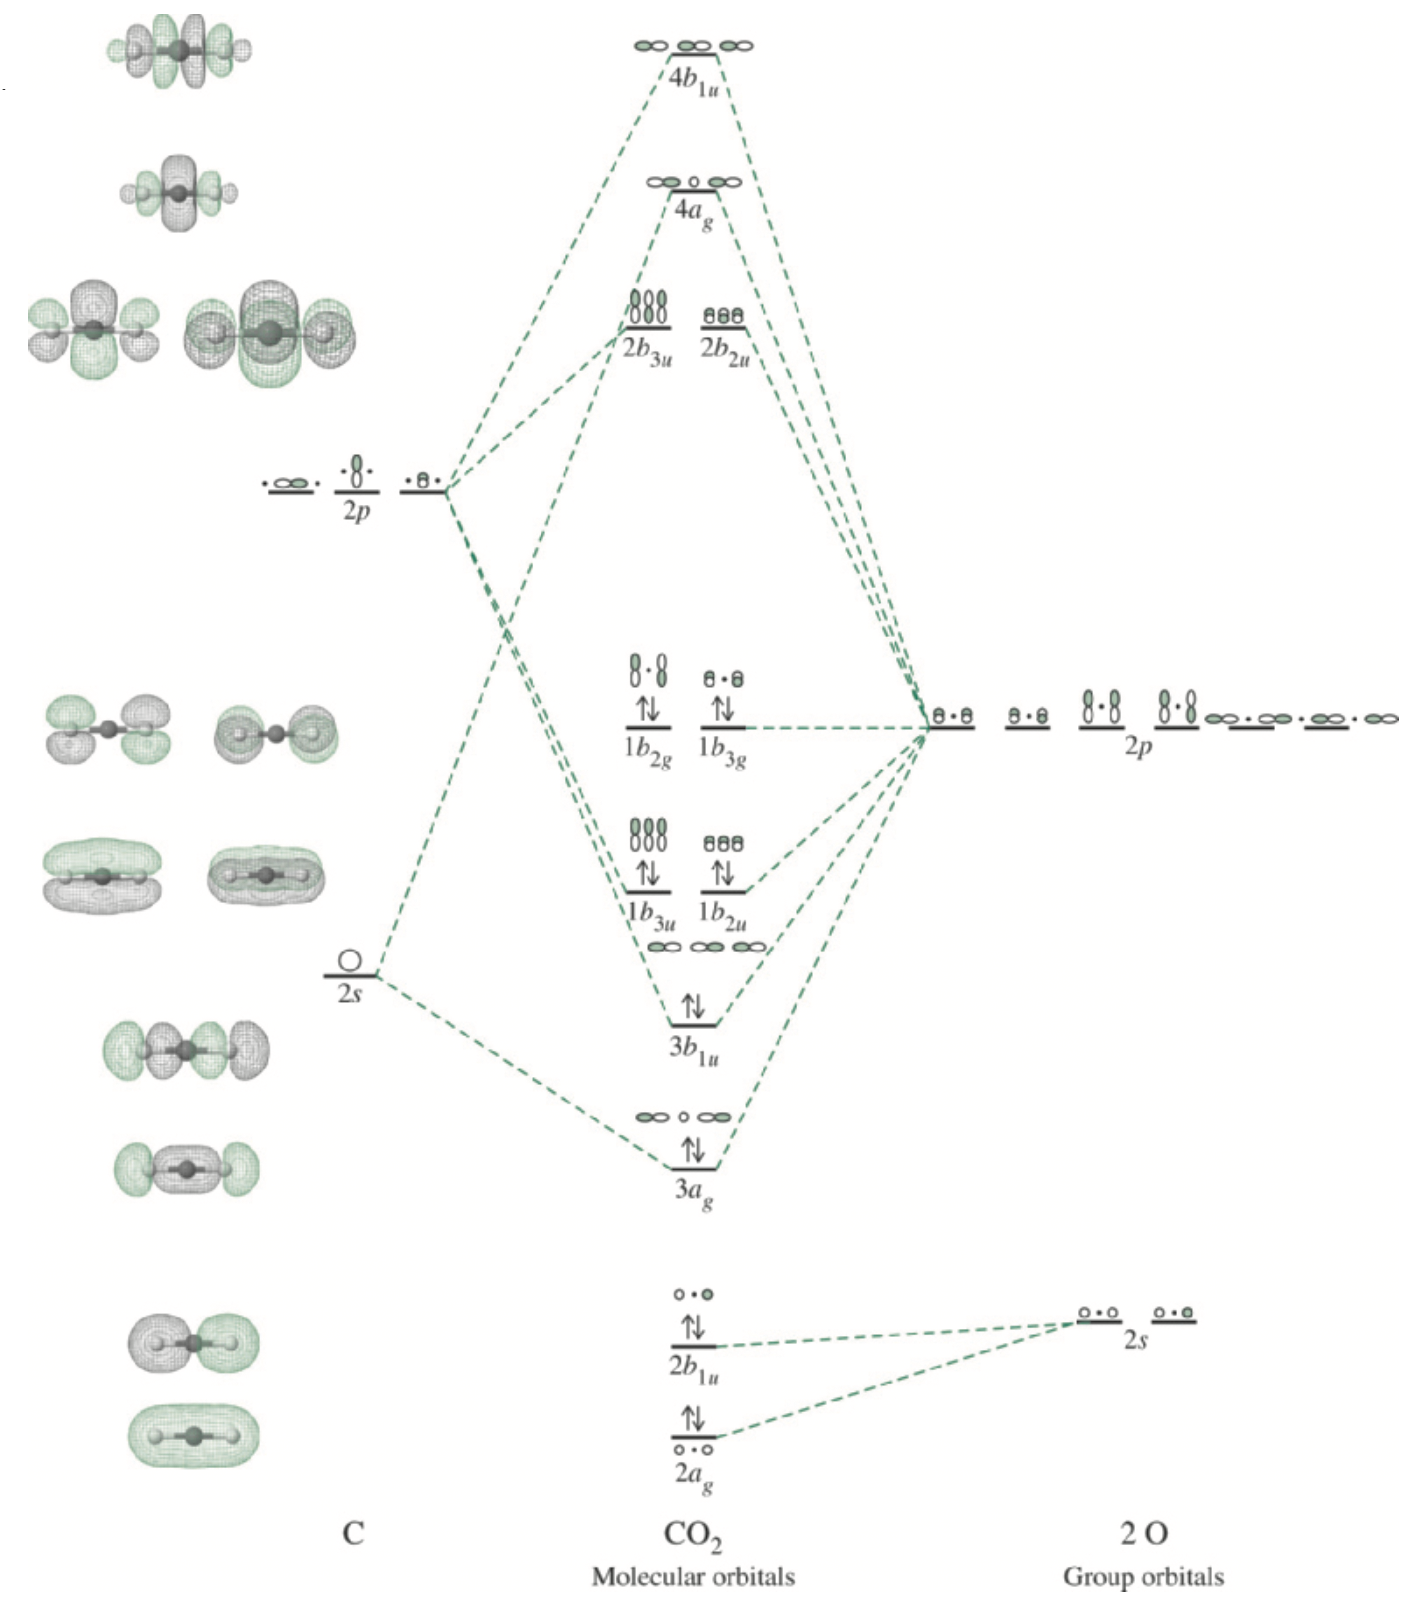
\includegraphics[width=0.8\linewidth]{../ExtFiles/molecularOrbitals-CO2.png}
        \caption{Molecular orbitals for \ce{CO2}.}
        \label{fig:molecularOrbitals-CO2}
    \end{figure}
    \begin{itemize}
        \item We find the same group orbitals as in \ce{FHF-} but by using the stepwise procedure.
        \begin{itemize}
            \item Note that saying $\Gamma_{2s}=A_g+B_{1u}$, for example, expresses the fact that there are two $2s$ orbitals (the sum and difference of the \ce{O}($2s$) orbitals) and that one has $A_g$ symmetry while the other has $B_{1u}$ symmetry.
        \end{itemize}
        \item The orbitals on the central atom are $2s,2p_z,2p_x,2p_y$.
        \item The $A_g$ \ce{O}($2s$) orbital can be added to and subtracted from the \ce{C}($2s$) orbital, and the $B_{1u}$ \ce{O}($2s$) orbital can be added to and subtracted from the \ce{C}($2p_z$) orbital.
        \begin{itemize}
            \item However, due to the large energy difference between the \ce{O} and \ce{C} orbitals, these do not generally form and are not included in Figure \ref{fig:molecularOrbitals-CO2}.
            \item Instead, the two \ce{O}($2s$) orbitals are included as $\sigma$ $2a_g$ and $2b_{1u}$, respectively, nonbonding orbitals.
        \end{itemize}
        \item The $A_g$ \ce{O}($2p_z$) orbital can be added to and subtracted from the \ce{C}($2s$) orbital, and the $B_{1u}$ \ce{O}($2p_z$) orbital can be added to and subtracted from the \ce{C}($2p_z$) orbital.
        \begin{itemize}
            \item From the first interaction: The $\sigma$ $3a_g$ bonding orbital formed is the most stable, with only two nodes and an uninterrupted probability region between the three nuclei. The $\sigma^*$ $4a_g$ antibonding orbital is the second least stable with four nodes.
            \item From the second interaction: The $\sigma$ $3b_{1u}$ bonding orbital formed is the second most stable, with only three nodes. The $\sigma^*$ $4b_{1u}$ antibonding orbital is the least stable with a whopping five nodes.
        \end{itemize}
        \item The $B_{2u}$ \ce{O}($2p_y$) orbital can be added to and subtracted from the \ce{C}($2p_y$) orbital, yet the $B_{3g}$ \ce{O}($2p_y$) orbital does not have matching symmetry with any \ce{C} orbital.
        \begin{itemize}
            \item From the first interaction: The $\pi$ $1b_{2u}$ bonding orbital formed is less stable than the $\sigma$ $3b_{1u}$ orbital since it lacks such direct probability between the nuclei but also has few nodes. The $\pi^*$ $2b_{2u}$ antibonding orbital is more stable than the $\sigma^*$ $4a_g$ antibonding orbital since it has fewer nodes.
            \item From the second interaction: The $\pi$ $1b_{3g}$ nonbonding orbital formed resides in the middle of the energy diagram.
        \end{itemize}
        \item The $B_{3u}$ \ce{O}($2p_x$) orbital can be added to and subtracted from the \ce{C}($2p_x$) orbital, yet the $B_{2g}$ \ce{O}($2p_x$) orbital does not have matching symmetry with any \ce{C} orbital.
        \begin{itemize}
            \item The cases are symmetric to the previous two.
        \end{itemize}
    \end{itemize}
    \item This process may be used to obtain numerical values for the coefficients of the atomic orbitals, but the computational methods are beyond the scope of \textcite{bib:MiesslerFischerTarr}.
    \item \ce{H2O} example:
    \begin{itemize}
        \item We canonically select that $xz$-plane as the plane of the molecule when we have a choice.
        \item Because the \ce{H}($1s$) orbitals have no directionality, it is not necessary to assign coordinate axes to the hydrogen atoms.
        \begin{table}[h!]
            \centering
            \renewcommand{\arraystretch}{1.6}
            \setlength{\tabcolsep}{1mm}
            \small
            \begin{tabular}{lccccll}
                \rowcolor{grx}
                \textcolor{white}{\textbf{Symmetry}} & \begin{tabular}{l}\textcolor{white}{\textbf{Molecular}}\\[-5pt]\textcolor{white}{\textbf{Orbitals}}\end{tabular} & & \begin{tabular}{l}\textcolor{white}{\textbf{Oxygen Atomic}}\\[-5pt]\textcolor{white}{\textbf{Orbitals}}\end{tabular} & & \begin{tabular}{l}\textcolor{white}{\textbf{Group Orbitals from}}\\[-5pt]\textcolor{white}{\textbf{Hydrogen Atoms}}\end{tabular} & \textcolor{white}{\textbf{Description}}\\
        
                $B_1$ & $\Psi_6$ & $=$ & $c_9\psi(p_x)$ & $+$ & $c_{10}[\psi(\ce{H}_a)-\psi(\ce{H}_b)]$ & Antibonding ($c_{10}$ is negative)\\
        
                \rowcolor{grt}
                $A_1$ & $\Psi_5$ & $=$ & $c_7\psi(s)$ & $+$ & $c_8[\psi(\ce{H}_a)+\psi(\ce{H}_b)]$ & Antibonding ($c_8$ is negative)\\
        
                $B_2$ & $\Psi_4$ & $=$ & $\psi(p_y)$ & & & Nonbonding\\
        
                \rowcolor{grt}
                $A_1$ & $\Psi_3$ & $=$ & $c_5\psi(p_z)$ & $+$ & $c_6[\psi(\ce{H}_a)+\psi(\ce{H}_b)]$ & Slightly bonding ($c_6$ is small)\\
        
                $B_1$ & $\Psi_2$ & $=$ & $c_3\psi(p_x)$ & $+$ & $c_4[\psi(\ce{H}_a)-\psi(\ce{H}_b)]$ & Bonding ($c_4$ is positive)\\
        
                \rowcolor{grt}
                $A_1$ & $\Psi_1$ & $=$ & $c_1\psi(s)$ & $+$ & $c_2[\psi(\ce{H}_a)+\psi(\ce{H}_b)]$ & Bonding ($c_2$ is positive)\\
            \end{tabular}
            \caption{Molecular orbital equations for \ce{H2O}.}
            \label{tab:Psi-H2O}
        \end{table}
        \item Note that the nonbonding pairs afforded by the MO model are not equivalent as in the Lewis model.
    \end{itemize}
    \item \ce{NH3} example:
    \begin{itemize}
        \item Is it not a bit circular to assign the point group $C_{3v}$ and then later use Walsh diagrams to determine that it has a $C_{3v}$ structure?
        \item Here, we can no longer just add and subtract atomic orbitals. Instead, we must apply "the projection operator method, a systematic approach for deduction of group orbitals" \parencite[152]{bib:MiesslerFischerTarr}.
        \item This method illustrates how atomic orbitals should be combined to afford the SALCs that define the group orbitals.
        \item First, determine the impact of each point group symmetry operation (individually, not within classes) on one atomic orbital.
        \item Linear combinations of these atomic orbitals that match the symmetries of the group's irreducible representations can be obtained via (1) multiplication of each outcome by the characters associated with each operation for these irreducible representations, followed by (2) addition of the results.
        \item Finding $\text{SALC}(A_1)=\frac{1}{\sqrt{3}}[\Psi(\ce{H}_a)+\Psi(\ce{H}_b)+\Psi(\ce{H}_c)]$ and $\text{SALC}(E)=\frac{1}{\sqrt{6}}[2\Psi(\ce{H}_a)-\Psi(\ce{H}_b)-\Psi(\ce{H}_c)]$ is easy.
        \item Now SALC($E$) has $y$ symmetry (note that this means that choosing the \ce{H_{$a$}} that we did in Figure \ref{fig:coordinates-NH3} [i.e., the one lying along a coordinate axis] has simplified calculations). Thus, the other SALC should have $x$ symmetry.
        \item \ce{H_{$a$}} should not contribute to the new SALC because of the orthogonal node defined by the $yz$-plane (if it contributed, there would be no $yz$ node). Thus, only \ce{H_{$b$}} and \ce{H_{$c$}} can contribute, and we can deduce that their coefficients are $\frac{1}{\sqrt{2}}$ and $-\frac{1}{\sqrt{2}}$, respectively, to satisfy the normalization requirement while also leading to identical total contributions from all three $1s$ wave functions across the three group orbitals.
    \end{itemize}
    \item In the projection operator method, orbitals can become the inverses of other orbitals.
    \item \ce{BF3} example:
    \begin{figure}[h!]
        \centering
        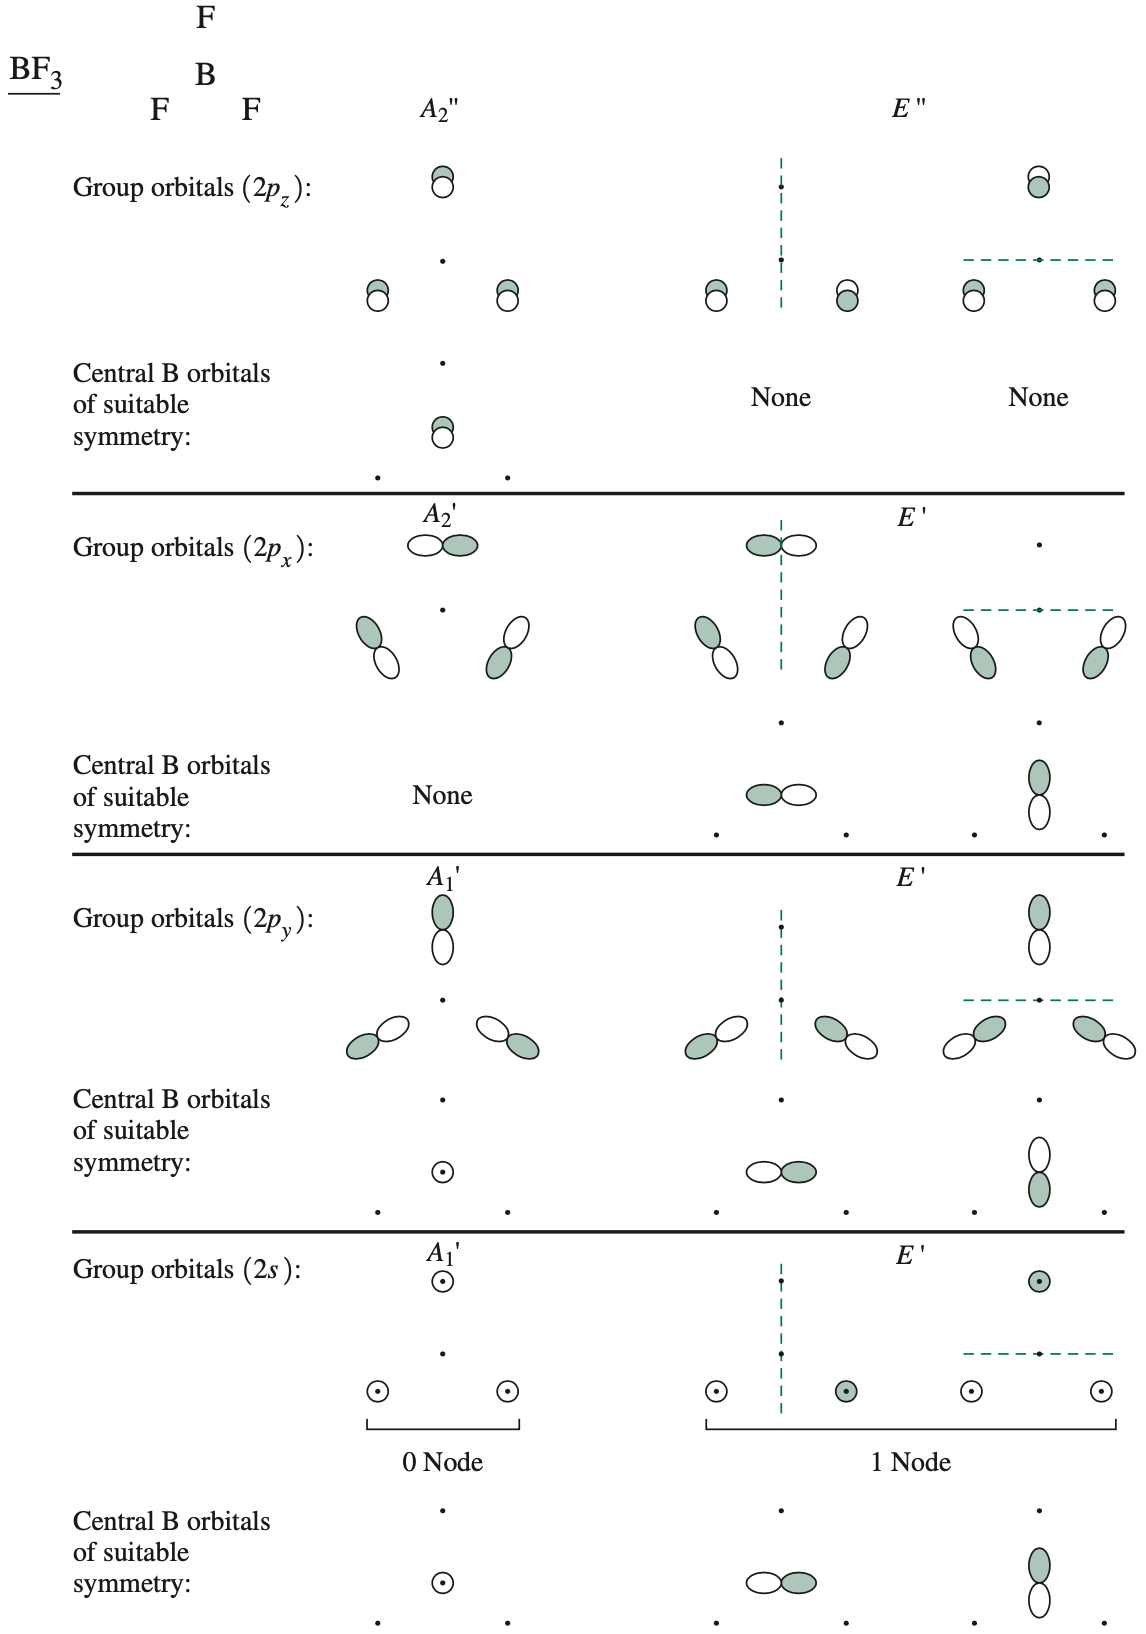
\includegraphics[width=0.7\linewidth]{../ExtFiles/groupOrbitals-BF3.png}
        \caption{Group orbitals for \ce{BF3}.}
        \label{fig:groupOrbitals-BF3}
    \end{figure}
    \begin{itemize}
        \item The fluorine ligands have $2p$ electrons, too, now. As such, let the $C_3$ axis be the $z$-axis, the $p_y$ axes point towards the central boron atom, and the $p_x$ axes lie in the molecular plane.
        \item The partial double bonding character of the \ce{B-F} bonds discussed in Chapter 3 can now be explained.
        \item The LUMO of \ce{BF3} is an empty antibonding $\pi$ orbital with large lobes on boron that can act as electron pair acceptors; this is why \ce{BF3} is a Lewis acid.
        \item This approach is also applicable to other isoelectronic trigonal planar species such as \ce{SO3}, \ce{NO3-}, and \ce{CO3^2-}.
    \end{itemize}
    \item "Because the extent of orbital overlap in $\pi$ interactions is generally less than that in most $\sigma$ interactions, a double bond composed of one filled $\sigma$ orbital and one filled $\pi$ orbital is not twice as strong as a single bond" \parencite[161]{bib:MiesslerFischerTarr}.
    \item Note that single bond energies between the same atoms can vary widely based on steric crowding and adjacent bonding.
    \item A qualitative group orbital approach (what we're doing) does not allow for the determination of the precise MO energies, but it generally allows for the placement of the MOs in the approximate order based on their shapes and expected orbital overlaps.
    \item "In the hybrid concept, the orbitals of the central atom are combined into sets of equivalent hybrids. These hybrid orbitals form bonds with orbitals of other atoms" \parencite[161]{bib:MiesslerFischerTarr}.
    \item Hybrid orbitals correctly describe methane's PES spectrum.
    \item "Like all bonding models, hybrids are useful so long as their limits are recognized" \parencite[161]{bib:MiesslerFischerTarr}.
    \item \ce{CH4} example:
    \begin{itemize}
        \item Point group: $T_d$.
        \item Basis functions: $\sigma$ bond vectors.
        \item $\Gamma=(4,1,0,0,2)$.
        \item $\Gamma=A_1+T_2$.
        \item "The atomic orbitals of carbon used in the hybrids must have symmetry matching $A_1+T_2$; more specifically, one orbital must match $A_1$, and a set of three (degenerate) orbitals must match $T_2$" \parencite[162]{bib:MiesslerFischerTarr}.
        \item For $A_1$, we choose the $2s$ orbital. For $T_2$, we could choose $d_{xy},d_{xz},d_{yz}$, but since they're much higher energy (and thus won't mix well with the \ce{H}($1s$) orbitals), we'll go for $p_x,p_y,p_z$.
        \item Therefore, the hybridization is $sp^3$, combining four atomic orbitals into four equivalent hybrid orbitals, one directed toward each hydrogen atom.
    \end{itemize}
    \item In addition to the $sp^3$ explanation of \ce{H2O}, it is sometimes explained through a slightly more MO theory lens as $sp^2$ since the oxygen orbitals used in MO bonding are $2s,2p_x,2p_z$ where the \ce{H2O} molecule lies in the $xz$-plane.
    \item Only $\sigma$ bonding is considered when determining the orbitals used in hybridization.
\end{itemize}




\end{document}